

%
%%
%%%The Grothendieck construction establishes an equivalence of categories between pseudofunctors from categories $\X$ into $\Cat$ and fibrations over $\X$.  There is a two-sided variation of this construction:
%%%
%%%
%%%\begin{theorem}{Benabou-Grothendieck}
%%%Take a lax normal functor $F:\mathcal{I}\to\Prof$ from a 1-category $\mathcal{I}$.
%%%
%%%Then the following pullback exists:
%%%$$
%%%\xymatrix{
%%%\int F \ar[d]_{} \ar[r]^{} & \Prof_*  \ar[d]\\
%%%\mathcal{I}^{\op} \ar[r] ^F          & \Prof
%%%}
%%%$$
%%%
%%%Where $\int F$ is a 1-category and $\int F \to \X$ is a functor.
%%%This extends to an isomorphism of categories:
%%%$$\int:\Cat_{l,n}(\X, \Prof)\cong \Cat/\X:\delta$$
%%%\end{theorem}
%%%
%%%$\Cat_{l,n}(\X, \Prof)$ is the category of lax normal functors from $\X$ to $\Prof$ and lax natural transformations. $\Cat/\X$ is the slice category over $\X$.
%%%
%%%
%%%Explicitly:
%%%\begin{lemma}
%%%$\int F$ has:
%%%\begin{description}
%%%\item[Objects:] Pairs $(Y \in \X_0, Y^\sharp \in F(Y))$
%%%\item[Morphisms:] 
%%%
%%%
%%%
%%%\item[Composition]
%%%\end{description}
%%%The functor $\int F\to \mathcal{I}^\op$ is the first projection from the pullback.
%%%
%%%\end{lemma}
%%%and conversely
%%%\begin{lemma}
%%%Given a functor $\delta: \mathcal{J}\to\mathcal{I}^\op$ $\delta \pi$ is the lax functor such that
%%%\begin{description}
%%%\item
%%%\item
%%%\itemend{description}
%%%\end{lemma}
%%%
%%%
%%%
%%%The Grothendieck construction has been extended to the monoidal case: establishing an equivalence between monoidal fibrations and monoidal pseudofunctors \cite[].  Similarly \cite[] prove the polycategorical Benabou-Grothendieck equivalence.  We adapt the work of both authors, by establishing a monoidal Grothendieck-Benabou equivalence:
%%%%
%%%%
%%%%
%%%%\begin{theorem}[Monoidal Grothendieck-Benabou construction.]
%%%%There is an equivalence of categories between the lax monoidal, lax normal functor category:
%%%%
%%%%\begin{description}
%%%%\item[Objects:]
%%%%\item[Maps:]
%%%%\item[Identity:]
%%%%\item[Composition:]
%%%%\end{description}
%%%%
%%%%and  the monoidal slice cateogry:
%%%%
%%%%\begin{description}
%%%%\item[Objects:]
%%%%\item[Maps:]
%%%%\item[Identity:]
%%%%\item[Composition:]
%%%%\end{description}
%%%%
%%%%\end{theorem}
%%%%\begin{proof}
%%%%Proof strategy: Start with a monoidal functor $\Y\to \X$ between strict monoidal categories.  Build a lax normal lax monoidal functor $\X\to \Prof$
%%%%
%%%%
%%%%Let $\X$ be a monoidal category, regarded as a monoidal bicategory with one object, and take a lax monoidal lax functor $F:\X\to\Prof$.  Then the following pullback exists in the category of monoidal bicategories, lax monoidal lax functors and lax natural transformations:
%%%%$$
%%%%\xymatrix{
%%%%\int F \ar[d]_{} \ar[r]^{} & \Prof_*  \ar[d]\\
%%%%\X \ar[r] ^F          & \Prof
%%%%}
%%%%$$
%%%%
%%%%$\int F$ has the same categorical structure as in the non-monoidal 
%%%%
%%%%
%%%%\end{proof}
%%%
%%%
%%%
%%%If $F$ is a normal frobenius monoidal lax normal functor
%%%with laxator $\ell$ monoidal laxator $\mu$ oplaxator $\nu$
%%%, then $\int F$ has an induced monoidal structure with:
%%%
%%% $F(X\otimes Y)\to F(X)\otimes F(Y) \to F(X')\otimes F(Y') \to F(X'\otimes Y')$
%%%
%%%\begin{description}
%%%\item[Tensor product:] On Objects:
%%%$$
%%%(Y,Y^\sharp) \otimes (Z,Z^\sharp)
%%%:=
%%%(Y\otimes Z, \nu(\mu(Y^\sharp, Z^\sharp)))
%%%$$
%%%
%%%On morphisms:
%%%$$
%%%(f,f^\sharp) \otimes (g,g^\sharp)
%%%:=
%%%(f\otimes g, \nu(\mu(f^\sharp, g^\sharp)) )
%%%$$
%%%
%%%\item[Tensor unit:]
%%%$$
%%%(I,* \in F(I))=\mathbb{1})
%%%$$
%%%\item[Unitors:]
%%%$$
%%%u_{(X,X^\sharp)}^R: (X,X^\sharp)\otimes (I,*)=(X\otimes I, \mu^{\otimes}(X^\sharp, *))  \to (X,X^\sharp)
%%%$$
%%%is given by
%%%$$
%%%(u_X^{R}:X\otimes I\to X,  f\in F(u_X^{R})(X^\sharp, \mu^{\otimes}(X^\sharp, *) )   )
%%%$$
%%%
%%%Where $f$ is the identity on $X$ along the isomorphism $ \mu^{\otimes}(X^\sharp, *) = $
%%%
%%%$
%%%(u_X^{R})(X^\sharp, X^\sharp)
%%%\cong
%%%(u_X^{R})(X^\sharp, \mu^{\otimes}(X^\sharp, *))
%%%$
%%%
%%%
%%%\item[Associator:]
%%%
%%%$$
%%%(\alpha_{X,Y,Z},  g):((X\otimes Y)\otimes Z, \mu^\otimes(\mu^{\otimes}(X^\sharp, Y^\sharp),Z^\sharp) \to 
%%%(X\otimes (Y\otimes Z),\mu^\otimes(X^\sharp, \mu^\otimes(Y^\sharp,Z^\sharp)))
%%%$$
%%%
%%%\end{description}
%%%
%%%
%%%Where the projection map $p:\int F\to\mathcal I$ moreover is strong monoidal:
%%%
%%%$$
%%%p ((X,X^\sharp )\times (Y,Y^\sharp )) = 
%%%$$
%%%
%%%
%%% Since we are regarding $\Prof$ as a quasistrict monoidal bicategory, if $\mathcal  I$ is strict monoidal, then so is $\int F$ so that the projection $\int F\to \mathcal I $ is strict monoidal.
%%%
%%%
%%%Conversely, suppose there is a strong monoidal functor $\pi:\mathcal{J}\to\mathcal{I}^\op$ between monoidal categories.
%%%Then $\delta \pi:\mathcal{I}^\op \to \Prof$ is a Frobenius monoidal, lax normal functor.  The monoidal laxators are given by:
%%%
%%%
%%%
%%%
%%%
%%%
%%%Given a monoidal category $p:\X\to \mathbb{1}$, the Frobenius monoidal lax structure of $\delta p : \mathbb{1}\to \Prof$ regarded as a lax monoidal functor is precisely the data of a representable lax special \dag-Frobenius algebra in $\Prof$:
%%%
%%%GIVE AXIOMS
%%%
%%%
%%%This is essentially the two-sided version of the coherence data of a monoidal category. 
%%%
%%%bicateggorical spider theorem
%%%
%%%Since $\mathbb{1}$ is strict monoidal, $\int \delta p$ is as well.
%%%Therefore we can deduce that this is the strictification of $\X$.
%%%
%%%Slice category definition of grothendieck construction
%%%
%%%Recalling the string diagrams for pointed profunctors, we have that the strictification of $\X$ is generated by.
%%%
%%%
%%%The monoidal Benabou-Grothendieck construction is a very general construction for creating string diagrams for the strictification of monoidal functors.  Given some algebraic structure $F$ in  $\Prof$, the lax normal, lax monoidal structure can be regarded as the data for a normal form.  Then each object in $\int F$ contains the information need
%%%
%%%
%%%
%%%
%%%
%%%
%%%
%%%
%%%
%%%
%%%
%%%
%%%
%%%
%%%
%%%
%%%
%%%
%%%
%%%
%%%
%%%
%%%
%%%
%%%
%%%
%%%
%%%
%%%Monoidal categories $\X$ are in bijection with pseudomonoids in Cat.
%%%These are in bijection with extraspecial representable dagger frobenius algebras in Prof
%%%which are in bijection with lax seperable normal dagger frobenius monoidal lax functors $F_\X:\mathbb{1}\to\Prof$.
%%%
%%%Since $\mathbb 1$ is strict monoidal so is $\int F_\X$.
%%%Moreover, there is a $\dag$-Frobenius monoidal pseudo functor $\iota:\X\to \Prof_*$ making the diagram commute:
%%%
%%%$$
%%%\xymatrix{
%%%\X  \ar[drr]^\iota \ar[ddr]  & &\\
%%%       &  \int F_\X \ar[d]_{} \ar[r]^{} & \Prof_*  \ar[d]\\
%%%       &  \mathbb{1} \ar[r] ^F          & \Prof
%%%}
%%%$$
%%%
%%%Therefore, the universal map $G:\X\to F_\X$ is a Frobenius monoidal pseudofunctor.  It can also be shown to be strong monoidal, and moreover an equivalence of categories.  Therefore $\int F_\X$ is the monoidal strictification of $\X$.
%%%
%%%
%%%This extends to an equivalence of categories:
%%%
%%%Monoidal functors $\X\to \Y$ are in bijection with pseudomonoid homomorphisms in Cat.  These are in bijection with monoidal natural transformations 
%%%$F_\X\Rightarrow F_\Y$.
%%%These are in bijection with strict monoidal functors $\int F_\X\to \int F_\Y$. These are in 
%%%
%%%Surely intertwiners between pseudomonoid homorphisms correspond to strict monoidal natural transformations.
%%%
%%%
%%%
%%%
%%%
%%%
%%%
%%%
%%%
%%%
%%%
%%%First show
%%%
%%%\begin{description}
%%%\item[0-cells:] Frobenius monoidal functors \mathcal{I}\to\Prof$
%%%\item[1-cells:] Frobenius monoidal lax natural transformations.
%%%\item[2-cells:] Intertwiners
%%%\end{description}
%%%
%%%is 2-equivalent
%%%
%%%\begin{description}
%%%\item[0-cells:] \int F
%%%\item[1-cells:] strong monoidal functors $\int F \to \int G$ making the triangle commute.
%%%\item[2-cells:] monoidal natural transformations
%%%\end{description}
%%%
%%%
%%%
%%%
%%%
%%%
%%%
%%%
%%%
%%%
%%%
%%%Consider the bicategory of:
%%%
%%%\begin{description}
%%%\item[0-cells:] Monoidal categories
%%%\item[1-cells:] Monoidal functors.
%%%\item[2-cells:] Monoidal natural transformations
%%%\end{description}
%%%
%%%is 2-isomorphic 
%%%
%%%\begin{description}
%%%\item[0-cells:] Pseudomonoids in Cat
%%%\item[1-cells:] Pseudomonoid homomorphisms.
%%%\item[2-cells:] Intertwiners
%%%\end{description}
%%%
%%%is 2-isomorphic 
%%%
%%%\begin{description}
%%%\item[0-cells:] XXX Frobenius pseudomonoid 
%%%\item[1-cells:] Pseudomonoid homomorphisms.
%%%Composition by conjugation
%%%\item[2-cells:] Intertwiners
%%%\end{description}
%%%
%%%is 2-isomorphic 
%%%
%%%\begin{description}
%%%\item[0-cells:] Frobenius monoidal functors $\mathbb{1}\to\Prof$
%%%\item[1-cells:] Frobenius monoidal lax natural transformations.
%%%\item[2-cells:] Intertwiners
%%%\end{description}
%%%
%%%is 2-equivalent
%%%
%%%\begin{description}
%%%\item[0-cells:] \int F
%%%\item[1-cells:] \alpha:\int F\to \int G
%%%\item[2-cells:] Intertwiners
%%%\end{description}
%%%
%%%is 2-isomorphic 
%%%
%%%\begin{description}
%%%\item[0-cells:] Strict monoidal categories
%%%\item[1-cells:] monoidal 
%%%\item[2-cells:] Intertwiners
%%%\end{description}
%%%
%%%
%%%
%%%
%%%
%%%
%%%
%%%
%%%
%%%Scalable ZX-calculus.
%%%
%%%hierarchical string diagrams
%%%
%%%
%%%
%%%
%%%
%%%Take the lax Frobenius monoidal $F:\N \to\Prof$
%%%sending $n=\prod_i p_i^{a_i }\mapsto \prod \Span(\Mat_{\F_{p_i}})$  for where the tensor in $\N$ is multiplication.
%%%
%%%
%%%There is a faithful functor $\int F\to\FHilb$ picking out phase free ZX diagrams with arbitrary finite dimension. This is because for the full subcategory off prime prower dimension $\int F |_p \hookrightarrow \int F$, $\int F |_p\cong \Span(\Mat_{\F_{p_i}})$. Moreover, the maps given by the laxators are change of basis vectors.
%%%
%%%
%%%
%%%If instead we do the same trick but sending $p$ to odd prime dimensional qudit complete-ZX diagrams, then we regain the qufinite presentation of the ZX-calculus of \cite{wang???}.
%%%
%%%
%%%
%%%For stabilizers, we can do the same modulo scalars, but with $F:\N/\{2\} \to\Prof$ picking out odd prime dimensional stabilizer diagrams.
%%%
%%%
%%
%%
%%
%%
%%
%%
%%
%%
%%
%%
%%
%%\begin{definition}
%%Given bicategories $\X$ and $\Y$, a lax normal functor $\X\to\Y$ is:
%%
%%TODO
%%\end{definition}
%%
%%
%%\begin{definition}
%%Given monoidal bicategories $\X$ and $\Y$, a  Frobenius monoidal lax normal functor is a lax normal functor $\X\to\Y$, equipped with 2-cells $\mu$ and $\nu$ called the monoidal laxator and oplaxators, and coherences called the left and right frobeniusators interacting with the compositors todo 
%%
%%TODO
%%\end{definition}
%%
%%
%%
%%\begin{definition}
%%A morphism between Frobenius monoidal lax normal functors $F,G\X\to\Y$ is.  Given two monoidal bicategories, this notion induces the Frobenius monoidal lax normal functor category, denoted $[\X,\Y]_{fln}$
%%\end{definition}
%%
%%\begin{lemma}
%%$[\X,\Y]_{fln}$ is a monoidal category with
%%\end{lemma}
%%
%%
%%
%%\begin{definition}
%%A monoidal displayed category is a monoidal category $\D$ equipped with a  Frobenius monoidal lax functor $\mathcal{D}\to\Prof$.
%%\end{definition}
%%
%%\begin{theorem}{Monoidal Grothendieck-Benabou construction}
%%Given a monoidal category $\X$, there is a monoidal equivalence between the Frobenius monoidal lax normal functor category $[\X,\Prof]_{fln}$ and the strict monoidal coslice category over $\X$.
%%\end{theorem}
%%
%%
%%
%%
%%
%%
%%
%%\begin{proof}
%%Fix a monoidal category $\X$.
%%
%%Take a strict monoidal functor $p:\Y\to\X$.
%%
%%
%%Given an object $X$ of $\X$, the indexed category of $p$ over $X$, $p^{-1}(X)$ has:
%%
%%Objects in $Y \in \Y$ such that $p^{-1}(Y)=X$.
%%
%%Morphisms $f:Y\to Y'$ such that $p^{-1}(f)=1_X$.
%%
%%Composition and identities in $\Y$.
%%
%%
%%Given a morphism $f:X\to X'$ to in $\X$, the reindexing profunctor $p^{-1}(f):p^{-1}(X)^\op  \times p^{-1}(X')\to \Set$ sends:
%%
%%objects: $p^{-1}(f)(Y,Y')= \{ g:Y\to Y' | p(g)=f \}$
%%maps: $p^{-1}(f)(h:Y\to Y', k:Z \to Z')=\lambda x \in p^{-1}(f)(Y,Y'). h;x;k$.
%%
%%
%%This has the structure of a lax normal functor $P^{-1}:\X\to\Prof$.
%%
%%
%%For objects $X,X',X'' \in \X$ the compositors at $X,X',X''$ at components $f:X\to X'$ and $g:X'\to X''$ are functions $\int^Z p^{-1}(f)(X,Z) \times p^{-1}(g)(Z,X'') \to  p^{-1}(f;g)(X,X'')$,
%%sending elements $(h,k)$ of the equivalence class to their composite $h;k$.  This is a function because $p(h;k) = p(h);p(k)=f;g$.
%%
%%
%%For each $X \in \X$, $p^{-1}(f)=1_X$ is the identity profunctor on $p^{-1}(X)$, so this functor is normal.
%%The desired commutative diagrams hold making this into a lax normal functor.
%%
%%Furthermore, we now show that this lax normal functor preserves the monoidal structure lax-Frobeniusly.
%%
%% 
%%
%%%1_{p^{-1}(X)} \to 
%%
%%%
%%%The components of the monoidal laxtator at $(f,g)$
%%%
%%%$$
%%%p^{-1}(f) \times p^{-1}(g) \Rightarrow p^{-1}(f \otimes g)
%%%$$
%%%
%%%are given by functions
%%%$$
%%%p^{-1}(f)\times p^{-1}(g) = \int^{Y} p^{-1}(f) (X,Y) \times p^{-1}(g) (W,Z)
%%%\Rightarrow 
%%%p^{-1}(f) (X,Y)\times p^{-1}(g) (W,Z)
%%%= \{h:X\to Y | p(h)=f \}\times  \{k: W\to Z | p(k)=g \}
%%%\Rightarrow
%%%\{\ell :X\otimes W \to Z \otimes Y | p(\ell)= f\otimes g  \}
%%%$$
%%%
%%%taking $(h,k) \mapsto h\otimes k$
%%%
%%%and oplaxator:
%%%
%%%$$
%%% p^{-1}(f \otimes g) \Rightarrow p^{-1}(f) \times p^{-1}(g)
%%%$$
%%%
%%%by functions:
%%%
%%%$$
%%% p^{-1}(f \otimes g)
%%%=
%%% \{h:X\to Y | p(h)=f\otimes g \}
%%%$$
%%%
%%
%%
%%
%%
%%The components of the monoidal laxtator at $(f:X\to X',g:X''\to X''')$
%%
%%$$
%%p^{-1}(f) \times p^{-1}(g) \Rightarrow p^{-1}(f \otimes g)
%%$$
%%
%%are given by functions 
%%sending elements $(h,k)\in p^{-1}(f)\times p^{-1}(g)$ to $h\otimes k \in p^{-1}(f \otimes g)$.  This is a function because $p(h\otimes k) = p(h)\otimes p(k)= h\otimes k$.
%%
%%
%%Unitor
%%
%%
%%
%%For the oplaxator at $(f:X\to X',g:X''\to X''')$
%%
%%
%%$$
%%p^{-1}(f \otimes g) \Rightarrow p^{-1}(f) \times p^{-1}(g)  
%%$$
%%are given by functions 
%%sending elements $h \in p^{-1}(f\otimes g)$
%%
%%
%%% $h;k$.  This is a function because $p(h;k) = p(h);p(k)=f;g$.
%%\end{proof}
%
%
%
%\newcommand{\Cat}{{\sf Cat}}
%
%In this Section, we will propose how to categorify categorical quantum mechanics by regarding monoidal categories themselves as a certain kind of special-commutative \dag-Frobenius algebra.  This will give a categorical account of proof nets for monoidal categories which we reviewed in the first Chapter.  This chapter is much more exploratory than the others, and indeed there is much more work that should be worked out in the future.
%
%
%We first need the following definition to motivate where we are going:
%
%\begin{definition}
%The symmetric monoidal bicategory of {\bf pointed Categories} is the coslice category $\Cat_*:=1/\Cat$.  Explicitly, this has:
%
%\begin{description}
%\item[0-cells:] A pointed category is a pair consisting of a category along with a chosen object of that category: 
%
%$$(\X, X\in\X_0)$$
%
%\item[1-cells:] A pointed functor between pointed categories is a pair consisting of a functor between the underlying categories and a morphism that preserves the points, as follows:
%
%$$(F:\X\to\Y, f\in \Y(F(X),Y) ):(\X, X\in\X_0)\to (\Y, Y\in\Y_0)$$
%
%\item[2-cells:] Given two parallel pointed functors, 
%
%$$
% (F:\X\to\Y, f\in \Y(F(X),Y) ),  (G:\X\to\Y, g\in \Y(G(X),Y) ):(\X, X\in\X_0)\to $(\Y, Y\in\Y_0)$
%$$
%
%a pointed natural transformation is natural transformation  $\phi:F\to G$ that preserves the distinguished map, so that $\phi_X:g=f$.
%\end{description}
%
%
%Composition of the 1-cells and 2-cells is given pointwise; and the monoidal structure is given by the Cartesian product.
%
%\end{definition}
%
%There is a graphical calculus for pointed categories.  If $\X$ is a monoidal category, then for every map $f:X\otimes Y\to Z$, there is a pointed functor:
%
%
%$$(\_\otimes \_ :\X^2\to\X, f\in \Y(F(X),Y) ):(\X^2, (X,Y)\in\X^2_0)\to (\X, Z\in\X_0)$$
%
%Drawn as follows:
%
%TODO DRAW
%
%
%Moreover, for every state $f:I\to X$, there is a pointed functor
%
%
%$$(I:1\to\X, f\in \Y(I,X) ):(1,* \in 1)\to (\X, I\in\X_0)$$
%
%
%
%Drawn as follows:
%
%DRAW
%
%
%
%Where $1$ is the strict monoidal category with one object and one morphism and $I:1\to \X$ is the functor which picks out the tensor unit and its identity in $\X$.
%
%
%Now, the pentagon equation means that the following diagram commutes:
%
%DRAW ASSOCIATOR WITH TREES AND ELEMENTS
%
%And the left and right unit equations mean that the following diagrams commute:
%
%DRAW LEFT AND RIGHT UNITORS WITH ELEMENTS 
%
%
%Instead of defining a monoidal category as we did in the first chapter, we could have instead defined a monoidal category as a pseudomonoid in $\Cat$.  Then the tensor product would become the multiplication and the tensor unit would become the unit:
%
%\begin{definition}
%Draw pseudomonoid coherences
%
%
%
%
%
%\end{definition}
%
%However, this does not generalize to other algenraic structures in $\Cat$.  For this we will need the following definition:
%
%
%\begin{definition}
%
%A {\bf pseudofunctor }
%A {\bf lax monoidal pseudofunctor}
%
%
%\end{definition}
%
%With this in mind, we have a concise definition of a monoidal category:
%
%
%\begin{lemma}
%A monoidal category is the data of a  lax monoidal pseudofunctor $:1\to \Cat$, where $1$ is the terminal monoidal category with one object and one morphism.
%\end{lemma}
%
%
%
%This definition may seem terse, as it moves around the coherence data into a different place; however, this is much more amenable to generalization.
%Indeed,  a {\bf monoidal indexed category} is a monoidal category $\X$ equipped with a lax monoidal functor $F:\X\to \Cat$.  
%
%
%\begin{definition}
%To every monoidal indexed category $F:\X\to \Cat$, the {\bf monoidal Grothendieck category} $\int F$ is a monoidal category with:
%
%
%\begin{description}
%
%\item[Objects: ]
%
%\item[Maps: ]
%
%Where the composition is:
%
%And the identity is:
%
%
%\item[Monoidal structure:]
%
%\end{description}
%
%\end{definition}
%
%
%Note the the projection  $\int F\to \X$ is strict monoidal.
%
%
%This projection is actually more than just a strict monoidal functor, it is a fibration!  In \cite{???}, they show that given a fixed monoidal category $\X$, the slice category of strict monoidal fibrations is equivalent to the lax monoidal pseudofunctor category from $\X\to \Cat$.  We wont discuss this further, because it is not immediately useful for our purposes.
%
%
%If we return to our working example $F_\X:1\to \Cat$ picking out a monoidal category, we find that there is a strict monoidal isomorhism between $\int F_\X$ and $\X$:
%
%TODO Draw composition and tensor product in terms of tubes.
%
%
%
%However, we could also take a different monoidal pseudofunctor into $\Cat$.
%
%\begin{definition}
%
%Given a monoidal category $\X$, define a strong monoidal pseudofunctor: $\Delta_\X:\Delta\to \Cat$
%
%sending $n\mapsto \X^n$, where the laxator left associates trees and eliminates units.
%
%\end{definition}
%
%Explicitly:
%
%\begin{lemma}
%$\int \Delta_\X$ is the strict monoidal category with:
%\begin{description}
%\item[Objects:] Finite lists of objects in $\X$.
%
%\item[Maps:]  Maps are binary forests, which are left associated where the units are elminated whenever possible.
%
%\item[Tensor:]  The tensor product is given by the cartesian product in pointed functors.
%
%\item[Composition:] The composition is given by nesting and then reducing the all connected components to the same normal form.
%
%
%\end{description}
%\end{lemma}
%
%
%However, this is a very one-sided construction, as the string diagrams in $\int \Delta_\X$ has the shapes of trees. 
%
%Draw laxator:
%
%
%One way to get around this is look at $\X$ as an object in $\Prof$, rather than $\Cat$.  There are two yoneda embeddings $y^* \Cat^\co \to \Prof$ and $y_*:\Cat^\op \to \Prof$.  Therefore, we can regard a monoidal category as both a pseudomonoid in $\Prof$ or a pseudocomonoid in $\Prof$. 
%
%
%
%\begin{definition}
%The monoidal bicategory of pointed profunctors, $\Prof_*$, has
%
%
%\begin{description}
%\item[0-cells:]
%
%\item[1-cells:]
%
%\item[2-cells:]
%\end{description}
%\end{definition}
%
%
%Pointed profunctors has a very similar graphical calculus to pointed categories.  Given a monoidal category one can regard not only factorizations of the domains of maps $f:X\otimes Y\to Z$, and states $g:I\to X$ as pointed profunctors, but also factorizations of the codomains of maps   $g:X \to Y\times Z$, and effects $h:X\to I$:
%
%
%TODO
%
%
%Now, it is known that autonomous monoidal categories correspond to pseudofrobenius algebras in prof which interact with the units and counits of the adjunctions between the the different components of the yoneda embedding, see \cite{???,???}.  However, the literature is quite terse and lacking; indeed, in the literature, many people miss this extra coherence equation governing the interaction of the pseudofrobenius algebra with the adjoints.  Moreover, a general monoidal category would not induce a pseudo frobenius algebra, but a Lax frobenius algebra. 
%
%The lax frobeniusators are given by the following 2-cells; which are hardly ever going to be invertible:
%
%TODO
%
%Given a monoidal category $\X$, it is therefore and open question as to what notion of functor is needed to regard the monoidal structure of  $\X$ as some sort of monoidal functor $1\to\Prof$.  There are lots of coherence equations to work out, but I conjecture that it is a lax normal functor that is lax monoidal and oplax monoidal such that the lax and oplax structures interact to form a lax frobenius algebra where the monoidal lax structure  is XXXX adjoint to the oplax structure. 
%
%
%As much as it would be nice to complete the picture, we don't really need this.  
%
%\begin{definition}
%Given a category $\X$ and a bicategory $\Y$, a lax normal functor is a pseudofunctor where the compositors are no longer required to be isomorphisms.
%A {\bf displayed category } is a category $\X$ equipped with a lax normal functor $\X\to \Prof$.
%\end{definition}
%
%\begin{lemma}
%Given a displayed category $F:\X\to \Prof$, the Grothendieck-Benabou category $\Pi \X$ has:
%
%\begin{description}
%\item[Objects:]
%\item[Maps:]
%\item[Composition:]
%\item[Identities:]
%\end{description}
%
%
%\end{lemma}
%
%
%Moreover, the projection $\Pi \X\to \X$ is a functor.  Given some fixed category $\X$, the correspondence extends between an equivalence of categories between the lax normal functor category from $\X$ to $\Prof$ and the slice category over $\X$.  This correspondence exists in several places in the literature and is thought to be due to Benabou.  It has recently started being called the Grothendieck-Benabou construction.
%
%
%\begin{lemma}
%Take a displayed category $F:\X\to \Prof$ such that $\X$ is monoidal and $F$ has the structure of a strong monoidal 2-functor.
%
%Then $\Pi \X$ has a monoidal structure given by:
%
%\end{lemma}
%
%
%%%%%This is where the important stuff is
%
%\begin{defintion}
%Given a monoidal category $\X$, there is a strong monoidal lax functor $G_\X:frob\to \Prof$ with
%
%\begin{description}
%\item[Objects:] $n\mapsto \X^n$
%\item[Compositor:] 
%\item[Unitor:] 
%\item[Tensorator:] 
%\item[Tensor-unitor:] 
%\end{description}
%
%
%\end{defintion}
%
%
%\begin{lemma}
%The Grothendieck benabou category $\Pi_\X$ is monoidal with:
%
%
%\begin{description}
%\item[Objects:] Finite lists of objects in $\X$.
%
%\item[Maps:] Two-sided forests in spider normal form, alongside elements:
%
%\item[Composition:] Composition is given by spider fusion of shapes.
%
%\item[Tensor:] The tensor product is given by the cartesian product in pointed profunctors.
%
%
%
%\end{description}
%\end{lemma}
%
%Proof nets live within the subcategory whose shapes are connected.  To actually get things to be connected, we have to force things to be connected:
%
%
%\begin{lemma}
%
%we can define a different tensor product on this category that squeezed to top and bottom wires together:
%
%\begin{definition}
%Given an object $X=[X_0,\cdots, X_{n-1}]$, define the projector on $X$ to be the map which inserts identities into the following diagram:
%
%Take the full subcategory of the Karoubi envelope, $\Lambda \X$, consisting of these projectors.
%
%This is the same as pr
%\end{definition}
%
%
%
%
%
%
%
%
%
%
%
%
%
%
%
%
%
%
%
%
%
%
%
%
%
%
%
%
%
%
%
%
%
%
%
%
%
%
%
%
%
%
%
%
%
%

In this Chapter, we attempt a high-level reconstruction of  proof nets by categorifying Frobenius algebras and appealing to a conjectural categorified spider theorem.  Starting with a monoidal category, we obtain a monoidal category which is not itself the strictification, but which is closely related.

We  hope that the highly conceptual level of the construction opens up avenues for finding string diagrams for more general algebraic structures; our goal being to find canonical ways to glue monoidal categories together and obtain new kinds of string diagrams thereof.  This kind of problem has previously been considered in the setting where one wants to glue together monoidal categories along multiple different monoidal functors \cite{lobski}.  The motivation therein is to give a semantics for ways to explain systems which are stratified into multiple different layers, although they obtain a monoidal bicategory, rather than an ordinary monoidal category where one has to keep track of coherence information.


Indeed, throughout this thesis, we have been drawing string diagrams in monoidal, or symmetric monoidal categories in which our familiar notions of monoids and Frobenius algebras and so on live.  However, if we move to the higher dimensional setting of monoidal bicategories, all of the equalities defining the axioms for these structures become natural transformations subject to  coherence conditions.   


For this Chapter, unlike the rest, I will assume that the reader has some familiarity with monoidal bicategories.


\section{Pointed categories and multicategories}

 First, we categorify a monoid in a monoidal category:

\begin{definition}
A {\bf pseudomonoid} in a monoidal bicategory is an object $\mathcal C$ equipped with two 1-cells ${C} \otimes \mathcal{C} \to \mathcal{C}$ and $\one \to \mathcal C$ drawn as follows:
$$
\begin{tikzpicture}
	\begin{pgfonlayer}{nodelayer}
		\node [style=Z] (4) at (2.5, 0) {};
		\node [style=none] (5) at (2.5, 1) {};
		\node [style=none] (6) at (2, -1) {};
		\node [style=none] (7) at (3, -1) {};
		\node [style=Z] (11) at (4.5, 0) {};
		\node [style=none] (12) at (4.5, 1) {};
		\node [style=none] (14) at (3.5, 0) {$,$};
	\end{pgfonlayer}
	\begin{pgfonlayer}{edgelayer}
		\draw [in=-135, out=90] (6.center) to (4);
		\draw (4) to (5.center);
		\draw [in=-45, out=90] (7.center) to (4);
		\draw (11) to (12.center);
	\end{pgfonlayer}
\end{tikzpicture}
$$





 as well as three 2-cells, the associator, left and right unitors:

$$
\begin{tikzpicture}
	\begin{pgfonlayer}{nodelayer}
		\node [style=Z]  (0) at (4, 0) {};
		\node [style=Z]  (1) at (4.5, 1) {};
		\node [style=none] (2) at (3.5, -1) {};
		\node [style=none] (3) at (4.5, -1) {};
		\node [style=none] (4) at (5.5, -1) {};
		\node [style=none] (5) at (4.5, 2) {};
		\node [style=Z]  (6) at (7.5, 0) {};
		\node [style=Z]  (7) at (7, 1) {};
		\node [style=none] (8) at (8, -1) {};
		\node [style=none] (9) at (7, -1) {};
		\node [style=none] (10) at (6, -1) {};
		\node [style=none] (11) at (7, 2) {};
		\node [style=none] (12) at (5.75, 1) {$\xRightarrow{\alpha}$};
		\node [style=Z]  (13) at (9.5, 1) {};
		\node [style=none] (15) at (10, 0) {};
		\node [style=none] (16) at (9, 0) {};
		\node [style=none] (18) at (9.5, 1.75) {};
		\node [style=Z]  (19) at (9, 0) {};
		\node [style=none] (20) at (10.25, 1) {$\xRightarrow{u^L}$};
		\node [style=Z]  (21) at (12.5, 1) {};
		\node [style=none] (22) at (12, 0) {};
		\node [style=none] (23) at (13, 0) {};
		\node [style=none] (24) at (12.5, 1.75) {};
		\node [style=Z]  (25) at (13, 0) {};
		\node [style=none] (26) at (11.75, 1) {$\xLeftarrow{u^R}$};
		\node [style=none] (27) at (11, 1.75) {};
		\node [style=none] (28) at (11, 0) {};
		\node [style=none] (29) at (8.25, 0.75) {,};
	\end{pgfonlayer}
	\begin{pgfonlayer}{edgelayer}
		\draw [in=90, out=-135] (0) to (2.center);
		\draw [in=-45, out=90] (3.center) to (0);
		\draw [in=-135, out=90] (0) to (1);
		\draw (1) to (5.center);
		\draw [in=-45, out=90] (4.center) to (1);
		\draw [in=90, out=-45] (6) to (8.center);
		\draw [in=-135, out=90] (9.center) to (6);
		\draw [in=-45, out=90] (6) to (7);
		\draw (7) to (11.center);
		\draw [in=-135, out=90] (10.center) to (7);
		\draw [in=90, out=-45] (13) to (15.center);
		\draw [in=-135, out=90] (16.center) to (13);
		\draw (13) to (18.center);
		\draw [in=90, out=-135] (21) to (22.center);
		\draw [in=-45, out=90] (23.center) to (21);
		\draw (21) to (24.center);
		\draw (28.center) to (27.center);
	\end{pgfonlayer}
\end{tikzpicture}
$$

Satisfying the maclane pentagon coherence equation (where the dashed blue box indicates where the nonidentity natural transformation is being applied):

$$
\begin{tikzpicture}
	\begin{pgfonlayer}{nodelayer}
		\node [style=none] (0) at (3.5, -4) {};
		\node [style=none] (1) at (4, -4) {};
		\node [style=none] (2) at (4.5, -4) {};
		\node [style=none] (3) at (5, -4) {};
		\node [style=none] (4) at (4.25, -1.5) {};
		\node [style=Z] (5) at (4.25, -3.25) {};
		\node [style=Z] (6) at (3.75, -2.75) {};
		\node [style=Z] (7) at (4.25, -2.25) {};
		\node [style=none] (8) at (2.75, -2.5) {$\xRightarrow{\alpha}$};
		\node [style=none] (9) at (5.75, -4) {};
		\node [style=none] (10) at (6.25, -4) {};
		\node [style=none] (11) at (6.75, -4) {};
		\node [style=none] (12) at (7.25, -4) {};
		\node [style=none] (13) at (6.5, -1.5) {};
		\node [style=Z] (14) at (6.5, -3.25) {};
		\node [style=Z] (15) at (6.5, -2.25) {};
		\node [style=none] (16) at (5.25, -2.5) {$\xRightarrow{\alpha}$};
		\node [style=Z] (17) at (7, -2.75) {};
		\node [style=none] (18) at (8, -2.5) {$\xRightarrow{\alpha}$};
		\node [style=none] (19) at (2.75, 0.75) {$\xRightarrow{\alpha}$};
		\node [style=none] (20) at (5.5, 0.75) {$\cong$};
		\node [style=none] (21) at (8, 0.75) {$\xRightarrow{\alpha}$};
		\node [style=none] (22) at (1.75, -3.5) {};
		\node [style=none] (23) at (1.75, -2.5) {};
		\node [style=none] (24) at (0.5, -2.5) {};
		\node [style=none] (25) at (0.5, -3.5) {};
		\node [style=none] (26) at (4.5, -3) {};
		\node [style=none] (27) at (4.5, -2) {};
		\node [style=none] (28) at (3.5, -2) {};
		\node [style=none] (29) at (3.5, -3) {};
		\node [style=none] (30) at (7.5, -3.5) {};
		\node [style=none] (31) at (7.5, -2.5) {};
		\node [style=none] (32) at (6.25, -2.5) {};
		\node [style=none] (33) at (6.25, -3.5) {};
		\node [style=none] (34) at (3.25, -0.75) {};
		\node [style=none] (35) at (3.75, -0.75) {};
		\node [style=none] (36) at (4.25, -0.75) {};
		\node [style=none] (37) at (4.75, -0.75) {};
		\node [style=Z] (38) at (3.5, 0) {};
		\node [style=Z] (39) at (4.5, 0.5) {};
		\node [style=Z] (40) at (4, 1) {};
		\node [style=none] (41) at (4, 1.75) {};
		\node [style=none] (42) at (5, -0.25) {};
		\node [style=none] (43) at (5, 0.75) {};
		\node [style=none] (44) at (3.25, 0.75) {};
		\node [style=none] (45) at (3.25, -0.25) {};
		\node [style=none] (46) at (7, 0.25) {};
		\node [style=none] (47) at (7, 1.25) {};
		\node [style=none] (48) at (6, 1.25) {};
		\node [style=none] (49) at (6, 0.25) {};
		\node [style=none] (50) at (2.25, 0.25) {};
		\node [style=none] (51) at (2.25, 1.25) {};
		\node [style=none] (52) at (1, 1.25) {};
		\node [style=none] (53) at (1, 0.25) {};
		\node [style=none] (54) at (6, -0.75) {};
		\node [style=none] (55) at (6.5, -0.75) {};
		\node [style=none] (56) at (7, -0.75) {};
		\node [style=none] (57) at (7.5, -0.75) {};
		\node [style=Z] (58) at (6.25, 0.5) {};
		\node [style=Z] (59) at (7.25, 0) {};
		\node [style=Z] (60) at (6.75, 1) {};
		\node [style=none] (61) at (6.75, 1.75) {};
		\node [style=none] (62) at (10, -0.5) {};
		\node [style=none] (63) at (9.5, -0.5) {};
		\node [style=none] (64) at (9, -0.5) {};
		\node [style=none] (65) at (8.5, -0.5) {};
		\node [style=Z] (66) at (9.75, 0.25) {};
		\node [style=Z] (67) at (9.25, 0.75) {};
		\node [style=Z] (68) at (8.75, 1.25) {};
		\node [style=none] (69) at (8.75, 2) {};
		\node [style=none] (70) at (1.5, -1.25) {$\shortparallel$};
		\node [style=none] (71) at (9.25, -1.25) {$\shortparallel$};
		\node [style=none] (72) at (10, -4) {};
		\node [style=none] (73) at (9.5, -4) {};
		\node [style=none] (74) at (9, -4) {};
		\node [style=none] (75) at (8.5, -4) {};
		\node [style=Z] (76) at (9.75, -3.25) {};
		\node [style=Z] (77) at (9.25, -2.75) {};
		\node [style=Z] (78) at (8.75, -2.25) {};
		\node [style=none] (79) at (8.75, -1.5) {};
		\node [style=none] (80) at (0.5, -4) {};
		\node [style=none] (81) at (1, -4) {};
		\node [style=none] (82) at (1.5, -4) {};
		\node [style=none] (83) at (2, -4) {};
		\node [style=Z] (84) at (0.75, -3.25) {};
		\node [style=Z] (85) at (1.25, -2.75) {};
		\node [style=Z] (86) at (1.75, -2.25) {};
		\node [style=none] (87) at (1.75, -1.5) {};
		\node [style=none] (88) at (0.5, -0.75) {};
		\node [style=none] (89) at (1, -0.75) {};
		\node [style=none] (90) at (1.5, -0.75) {};
		\node [style=none] (91) at (2, -0.75) {};
		\node [style=Z] (92) at (0.75, 0) {};
		\node [style=Z] (93) at (1.25, 0.5) {};
		\node [style=Z] (94) at (1.75, 1) {};
		\node [style=none] (95) at (1.75, 1.75) {};
	\end{pgfonlayer}
	\begin{pgfonlayer}{edgelayer}
		\draw [in=90, out=-60] (5) to (2.center);
		\draw [in=-120, out=90] (1.center) to (5);
		\draw (5) to (6);
		\draw [in=-165, out=90] (6) to (7);
		\draw (7) to (4.center);
		\draw [in=90, out=-45, looseness=0.75] (7) to (3.center);
		\draw [in=90, out=-120] (6) to (0.center);
		\draw [in=90, out=-60] (14) to (11.center);
		\draw [in=-120, out=90] (10.center) to (14);
		\draw (15) to (13.center);
		\draw [in=90, out=-165] (17) to (14);
		\draw [in=-45, out=90, looseness=0.75] (12.center) to (17);
		\draw (17) to (15);
		\draw [in=90, out=-150] (15) to (9.center);
		\draw [color=blue,dashed] (22.center) to (23.center) to (24.center) to (25.center) to cycle;
		\draw [color=blue,dashed] (26.center) to (27.center) to (28.center) to (29.center) to cycle;
		\draw [color=blue,dashed] (30.center) to (31.center) to (32.center) to (33.center) to cycle;
		\draw [in=90, out=-60] (38) to (35.center);
		\draw [in=90, out=-120] (38) to (34.center);
		\draw (41.center) to (40);
		\draw [in=90, out=-15] (40) to (39);
		\draw [in=90, out=-60] (39) to (37.center);
		\draw [in=-120, out=90] (36.center) to (39);
		\draw [in=90, out=-135] (40) to (38);
		\draw [color=blue,dashed] (42.center) to (43.center) to (44.center) to (45.center) to cycle;
		\draw [color=blue,dashed] (46.center) to (47.center) to (48.center) to (49.center) to cycle;
		\draw [color=blue,dashed] (50.center) to (51.center) to (52.center) to (53.center) to cycle;
		\draw [in=90, out=-60] (58) to (55.center);
		\draw [in=90, out=-120] (58) to (54.center);
		\draw (61.center) to (60);
		\draw [in=90, out=-45] (60) to (59);
		\draw [in=90, out=-60] (59) to (57.center);
		\draw [in=-120, out=90] (56.center) to (59);
		\draw [in=90, out=-165] (60) to (58);
		\draw [in=90, out=-120] (66) to (63.center);
		\draw [in=90, out=-60] (66) to (62.center);
		\draw (69.center) to (68);
		\draw [in=90, out=-15] (68) to (67);
		\draw [in=90, out=-15] (67) to (66);
		\draw [in=90, out=-120] (67) to (64.center);
		\draw [in=90, out=-120] (68) to (65.center);
		\draw [in=90, out=-120] (76) to (73.center);
		\draw [in=90, out=-60] (76) to (72.center);
		\draw (79.center) to (78);
		\draw [in=90, out=-15] (78) to (77);
		\draw [in=90, out=-15] (77) to (76);
		\draw [in=90, out=-120] (77) to (74.center);
		\draw [in=90, out=-120] (78) to (75.center);
		\draw [in=90, out=-60] (84) to (81.center);
		\draw [in=90, out=-120] (84) to (80.center);
		\draw (87.center) to (86);
		\draw [in=90, out=-165] (86) to (85);
		\draw [in=90, out=-165] (85) to (84);
		\draw [in=90, out=-60] (85) to (82.center);
		\draw [in=90, out=-60] (86) to (83.center);
		\draw [in=90, out=-60] (92) to (89.center);
		\draw [in=90, out=-120] (92) to (88.center);
		\draw (95.center) to (94);
		\draw [in=90, out=-165] (94) to (93);
		\draw [in=90, out=-165] (93) to (92);
		\draw [in=90, out=-60] (93) to (90.center);
		\draw [in=90, out=-60] (94) to (91.center);
	\end{pgfonlayer}
\end{tikzpicture}
$$


As well as the unit coherences:

$$
\begin{tikzpicture}
	\begin{pgfonlayer}{nodelayer}
		\node [style=none] (47) at (2.75, 0.75) {$\xRightarrow{\alpha}$};
		\node [style=none] (100) at (1.5, -1.25) {$\shortparallel$};
		\node [style=none] (120) at (0.75, -0.75) {};
		\node [style=none] (121) at (2.25, -0.75) {};
		\node [style=Z] (122) at (1.5, -0.25) {};
		\node [style=Z] (123) at (1.25, 0.5) {};
		\node [style=Z] (124) at (1.75, 1.25) {};
		\node [style=none] (125) at (1.75, 1.75) {};
		\node [style=none] (126) at (5, -0.5) {};
		\node [style=none] (127) at (5, 0.75) {};
		\node [style=none] (128) at (3.75, 0.75) {};
		\node [style=none] (129) at (3.75, -0.5) {};
		\node [style=none] (130) at (4.75, -0.75) {};
		\node [style=none] (131) at (3.25, -0.75) {};
		\node [style=Z] (132) at (4, -0.25) {};
		\node [style=Z] (133) at (4.25, 0.5) {};
		\node [style=Z] (134) at (3.75, 1.25) {};
		\node [style=none] (135) at (3.75, 1.75) {};
		\node [style=none] (136) at (2.25, 0.25) {};
		\node [style=none] (137) at (2.25, 1.5) {};
		\node [style=none] (138) at (1, 1.5) {};
		\node [style=none] (139) at (1, 0.25) {};
		\node [style=Z] (144) at (7.25, 0.75) {};
		\node [style=none] (145) at (7.25, 1.75) {};
		\node [style=none] (146) at (6.75, -0.75) {};
		\node [style=none] (147) at (7.75, -0.75) {};
		\node [style=none] (148) at (6, 0.75) {$\xRightarrow{ u^L}$};
		\node [style=none] (149) at (7.25, -1.25) {$\shortparallel$};
		\node [style=none] (150) at (0.5, -4.25) {};
		\node [style=none] (151) at (2, -4.25) {};
		\node [style=Z] (152) at (1.25, -3.75) {};
		\node [style=Z] (153) at (1, -3) {};
		\node [style=Z] (154) at (1.5, -2.25) {};
		\node [style=none] (155) at (1.5, -1.75) {};
		\node [style=none] (156) at (1.5, -4) {};
		\node [style=none] (157) at (1.5, -2.75) {};
		\node [style=none] (158) at (0.25, -2.75) {};
		\node [style=none] (159) at (0.25, -4) {};
		\node [style=none] (160) at (4.25, -3.25) {$\xRightarrow{u^R}$};
		\node [style=Z] (161) at (7.25, -3) {};
		\node [style=none] (162) at (7.25, -1.75) {};
		\node [style=none] (163) at (6.75, -4.25) {};
		\node [style=none] (164) at (7.75, -4.25) {};
	\end{pgfonlayer}
	\begin{pgfonlayer}{edgelayer}
		\draw (125.center) to (124);
		\draw [in=90, out=-165] (124) to (123);
		\draw [in=90, out=-45] (123) to (122);
		\draw [in=90, out=-135] (123) to (120.center);
		\draw [in=90, out=-45, looseness=0.75] (124) to (121.center);
		\draw [color=blue,dashed] (126.center) to (127.center) to (128.center) to (129.center) to cycle;
		\draw (135.center) to (134);
		\draw [in=90, out=-15] (134) to (133);
		\draw [in=90, out=-135] (133) to (132);
		\draw [in=90, out=-45] (133) to (130.center);
		\draw [in=90, out=-135, looseness=0.75] (134) to (131.center);
		\draw [color=blue,dashed] (136.center) to (137.center) to (138.center) to (139.center) to cycle;
		\draw (145.center) to (144);
		\draw [in=90, out=-45] (144) to (147.center);
		\draw [in=-135, out=90] (146.center) to (144);
		\draw (155.center) to (154);
		\draw [in=90, out=-165] (154) to (153);
		\draw [in=90, out=-45] (153) to (152);
		\draw [in=90, out=-135] (153) to (150.center);
		\draw [in=90, out=-45, looseness=0.75] (154) to (151.center);
		\draw [color=blue,dashed] (156.center) to (157.center) to (158.center) to (159.center) to cycle;
		\draw (162.center) to (161);
		\draw [in=90, out=-45] (161) to (164.center);
		\draw [in=-135, out=90] (163.center) to (161);
	\end{pgfonlayer}
\end{tikzpicture}
$$

A pseudomonoid is {\bf strict} when the associator and unitors are idenities.

\end{definition}

If we take $\Cat$ to be a monoidal bicategory with respect to the Cartesian product, then monoidal categories have a slick definition:

\begin{lemma}
Monoidal categories are pseudomonoids in $\Cat$ and strict monoidal categories are strict pseudomonoids in $\Cat$.
\end{lemma}

Contrast this with the view of small {\em strict} monoidal categories as categories internal to monoids between spans of sets; in the non-internal setting, the ability to express the pseudoness of the monoid allows the tensor product to not be strict.

By looking at the points inside of $\Cat$, this way of viewing a monoidal category hints at some connection to proof nets:

\begin{definition}
The symmetric monoidal bicategory of {\bf pointed categories} is the coslice bicategory $\Cat_*:=\one/\Cat$.  Explicitly, this has:

\begin{description}
\item[0-cells:] Pointed categories, pairs consisting of a category along with a chosen object of that category: 

$$(\X, X\in\X_0)$$

\item[1-cells:] Pointed functor between pointed categories,   pairs consisting of a functor between the underlying categories and a morphism that preserves the point:

$$(F:\X\to\Y, f\in \Y(F(X),Y) ):(\X, X\in\X_0)\to (\Y, Y\in\Y_0)$$

\item[2-cells:] Given two parallel pointed functors $(F,f),  (G,g):(\X,X)\to (\Y,X)$,
a pointed natural transformation is natural transformation  $\phi:F\to G$ that preserves the distinguished map, so that $\phi_X:g=f$.
\end{description}


Composition of the 1-cells and 2-cells is given pointwise; and the monoidal structure is given by the Cartesian product.

\end{definition}

There is a graphical calculus for pointed profunctors, which we will first specialize to pointed categories.  To my knowledge the graphical calculus is not fully worked out in the literature.  Initially called ``internal string diagrams''  by \cite{vicary} when applied to  $\Vect$-enriched Profunctors, these have also been called ``open diagrams'' by \cite{mario} for $\Sets$-enriched profunctors. We use the package contained in the paper \cite{vicary} to typeset these diagrams.  We will return to the case of $\Sets$-enriched profunctors shortly.

Given a pointed functor, $(1_\X, f \in \X(1_{\X}(X),Y))$, draw the identity as a cylinder and the map inside the cylinder as follows:


$$
\begin{tikzpicture}[scale=1.5]
    \node[Cyl, bot, top, height scale=1.0] (A) at (0,0) {};
    \begin{scope}[internal string scope]
        \node (i) at  ($(A.bot)+(0,-.3)$)  {\tiny $X$};
        \node (j) at ($(A.top)+(0,.3)$)  {\tiny $Y$};
        \node [tiny label] (g) at (A.center) {$f$};
        \draw (A.bot) to (A.top);
    \end{scope}
\end{tikzpicture}
$$
Think of the maps inside the category as ``living'' within the cylinder; wherein one can apply rewrite rules coming from the equational theory of the category.  

Functors are drawn as membranes between separating the cylinder for the domain and codomain category; functoriality means that things can pass up through the membrane:


$$
\begin{tikzpicture}[scale=1.5]
    \node[Cyl, bot, top,xscale=1.5,yscale=1.1] (A) at (0,0) {};
    \node[Cyl, bot, anchor=top,xscale=1.5,yscale=1.1] (B) at (A.bot) {};
    \node (g) at ($(A.bot)+(-.5,0)$) {\tiny $F$};
    \begin{scope}[internal string scope]
        \node (i) at  ($(B.bot)+(0,-.3)$)  {\tiny $X$};
        \node (j) at ($(A.top)+(0,.3)$)  {\tiny $F(Y)$};
        \node [tiny label] (g) at (B.center) {$f$};
        \draw (B.bot) to (A.top);
    \end{scope}
\end{tikzpicture}
=
\begin{tikzpicture}[scale=1.5]
    \node[Cyl, bot, top,xscale=1.5,yscale=1.1] (A) at (0,0) {};
    \node[Cyl, bot, anchor=top,xscale=1.5,yscale=1.1] (B) at (A.bot) {};
    \node (g) at ($(A.bot)+(-.5,0)$) {\tiny $F$};
    \begin{scope}[internal string scope]
        \node (i) at  ($(B.bot)+(0,-.3)$)  {\tiny $X$};
        \node (j) at ($(A.top)+(0,.3)$)  {\tiny $F(Y)$};
        \node [tiny label] (g) at (A.center) {$F(f)$};
        \draw (B.bot) to (A.top);
    \end{scope}
\end{tikzpicture}
$$

If $\X$ is a monoidal category, then one can tensor maps within the cobordism using the tensor product of $\X$, so that for $f:W\to X$ and $g:Y\to Z$, we have the the pointed functor  $(1_\X, f\times  \in \X(1_{\X}(W\otimes X),(Y\otimes Z)))$  with the following graphical representation:

$$
\begin{tikzpicture}[scale=1.5]
    \node[Cyl, bot, top,xscale=1.5,yscale=1.1] (A) at (0,0) {};
    \begin{scope}[internal string scope]
        \node [tiny label] (f) at ($(A.center)+(-.15,0)$) {$f$};
        \node [tiny label] (g) at ($(A.center)+(.15,0)$) {$g$};
        \draw ($(A.bot)+(-.15,0)$) to (f) to ($(A.top)+(-.15,0)$);
        \draw ($(A.bot)+(.15,0)$) to (g) to ($(A.top)+(.15,0)$) ;
        \node (i) at (A.top) [above] {\tiny $Y\otimes Z$};
        \node (j) at (A.bot) [below] {\tiny $W\otimes X$};
    \end{scope}
\end{tikzpicture}
$$

Moreover, for every map with a binary tensor factorization of the domain  $f:X\otimes Y\to Z$, we can use the external tensor product of $\Cat$ to obtain a pointed functor:

$$
(\_\otimes \_ :\X^2\to\X, f\in \Y(X\otimes Y ,Z) ):(\X^2, (X,Y)\in\X^2_0)\to (\X, Z\in\X_0)$$

Drawn as follows:

$$
\begin{tikzpicture}[scale=1.5]
    \node[Pants, bot, top, height scale=1.0] (A) at (0,0) {};
    \begin{scope}[internal string scope]
        \node (i) at (A.belt) [above] {\tiny $Z$};
        \node (j) at (A.leftleg) [below] {\tiny $X$};
        \node (k) at (A.rightleg) [below] { \tiny $Y$};
        \node [tiny label] (g) at (0,0.02\cobheight) {$f$};
        \draw (i.south)
            to (g.center)
            to [out=-140, in=up] (j.north);
        \draw (g.center)
            to [out=-40, in=up] (k.north);
    \end{scope}
\end{tikzpicture}
$$


And for every state $f:I\to X$, there is a pointed functor


$$(I:\one\to\X, f\in \Y(I,X) ):(1,* \in \one)\to (\X, I\in\X_0)$$



Drawn as follows:

$$
\begin{tikzpicture}[scale=1.5]
\setlength\cupheight{1.5\cupheight}
\node (i) at (0,0) [Cup, top] {};
\node (j) at (0,-\cobheight) [Bot3D, invisible] {};
\node (g) [tiny label] at (0,-0.4\cobheight) {$f$};
\begin{scope}[internal string scope]
\node (di) at (i.center) [above] {\tiny $A$};
\draw (i.center) to (g.center) {};
\end{scope}
\end{tikzpicture}
$$

Consider the action of the associator and unitor on the points:



$$
\begin{tikzpicture}[scale=1.5]
    \node[Pants, bot, top] (B) at (0,0) {};
    \node[Pants, bot, anchor=belt] (A) at (B.leftleg) {};
    \node[SwishL, bot, anchor=top] (C) at (B.rightleg) {};
    \begin{scope}[internal string scope]
        \node (i) at (B.belt) {};
        \node (j) at (A.leftleg){};
        \node (k) at (A.rightleg) {};
        \node (l) at (C.bot) {} ;
        \node [tiny label] (f) at (B.center) {$f$};
        \node [tiny label] (g) at (A.center) {$g$};
        \node [tiny label] (h) at (C.center) {$h$};
        \draw (f.center) to (i.center);
        \draw (j.center) to [out=up, in=-135] (g.center);
        \draw (k.center) to [out=up, in=-35] (g.center);
        \draw (g.center) to [out=90, in=-135] node [left=-4pt] {} (f.center);
        \draw (l.center)
            to [out=90, in=-80] (h.center) 
            to [out=up, in=down, out looseness=0.7]
                (B.rightleg)
            to [out=up, in=-45]
                node [right=-4pt, pos=0.11] {}
 (f.center);
    \end{scope}
    \end{tikzpicture}
    \xRightarrow{\alpha}
\begin{tikzpicture}[scale=1.5]
    \node[Pants, bot, top] (B) at (0,0) {};
    \node[Pants, bot, anchor=belt] (A) at (B.rightleg) {};
    \node[SwishR, bot, anchor=top] (C) at (B.leftleg) {};
    \begin{scope}[internal string scope]
        \node (i) at (B.belt) {};
        \node (j) at (C.bot)  {};
        \node (k) at (A.leftleg) {};
        \node (l) at (A.rightleg)  {};
        \node [tiny label] (f) at (0.05\cobwidth,0.18\cobheight) {$f$};
        \node [tiny label] (g)  at (-0.4\cobwidth,-0.1\cobheight) {$g$};
        \draw (j.center)
            to [out=up, in=-130] (g.center);
        \draw (k.center)
            to [out=up, in=down] (B-rightleg.in-leftthird)
            to [out=up, in=-40] (g.center);
        \draw (l.center) to [out=up, in=down] (B-rightleg.in-rightthird)
            to [out=up, in=-60] (f.center);
        \draw (f.center) to [out=90, in=-90, looseness=2] (i.center);
        \draw (f.center) to [in=90, out=-120] (g.center);
        \node [tiny label] (h) at (0.8\cobwidth,-0.25\cobheight) {$h$};
    \end{scope}
    \end{tikzpicture}\ ,
\hspace*{.5cm}
\begin{tikzpicture}[scale=1.5]
    \node[Pants, top, bot] (A) at (0,0) {};
    \node[Cup] (B) at (A.leftleg) {};
    \node[Cyl, bot, anchor=top] (C) at (A.rightleg) {};
    \begin{scope}[internal string scope]
        \node [tiny label] (f) at (0,0) {$f$};
        \node [tiny label] (g) at ([yshift=-0.3\cobheight] B) {$g$};
        \node [tiny label] (h) at (C) {$h$};
        \node (i) at (A.belt) [above] {};
        \node (i2) at (C.bottom) [below] {};
        \draw (f.center) to [out=-140, in=90] node [left=-3pt] {} (g.center);
        \draw (f.center) to (i);
        \draw (f.center)
            to [out=-40, in=90, looseness=0.9]
                node [right=-2pt, pos=0.4] {} (h.center);
        \draw (h.center) to (i2);
    \end{scope}
\end{tikzpicture}
\xRightarrow{u^L}
\begin{tikzpicture}[scale=1.5]
    \node[Cyl, tall, bot, top] (A) at (0,0) {};
    \begin{scope}[internal string scope]
        \node [tiny label] (f) at (0,0.4\cobheight) {$f$};
        \node [tiny label] (g) at (-0.20\cobwidth, -0.1\cobheight) {$g$};
        \node [tiny label] (h) at (0.20\cobwidth,-0.5\cobheight) {$h$};
        \node (i) at (A.top) [above] {};
        \node (i2) at (A.bot) [below] {};
        \draw (f.center) to [out=-120, in=90] (g.center);
        \draw (f.center) to (i);
        \draw (f.center)
            to [out=-60, in=90, looseness=0.9] (h.center);
        \draw (h.center) to [out=-90, in=up, looseness=1.2] (i2.north);
    \end{scope}
\end{tikzpicture}\ ,
\hspace*{.5cm}
\begin{tikzpicture}[scale=1.5]
    \node[Pants, top, bot] (A) at (0,0) {};
    \node[Cup] (B) at (A.rightleg) {};
    \node[Cyl, bot, anchor=top] (C) at (A.leftleg) {};
    \begin{scope}[internal string scope]
        \node [tiny label] (f) at (0,0) {$f$};
        \node [tiny label] (g) at ([yshift=-0.3\cobheight] B) {$g$};
        \node [tiny label] (h) at (C) {$h$};
        \node (i) at (A.belt) [above] {};
        \node (i2) at (C.bottom) [below] {};
        \draw (f.center) to [out=-40, in=90] node [right=-1pt] {} (g.center);
        \draw (f.center) to (i);
        \draw (f.center)
            to [out=-140, in=90, looseness=0.9]
                %node [left=-2pt, pos=0.4] {$Y$}
                (h.center);
        \draw (h.center) to (i2);
    \end{scope}
\end{tikzpicture}
\xRightarrow{u^R}
\begin{tikzpicture}[scale=1.5]
    \node[Cyl, tall, bot, top] (A) at (0,0) {};
    \begin{scope}[internal string scope]
        \node [tiny label] (f) at (0,0.4\cobheight) {$f$};
        \node [tiny label] (g) at (0.2\cobwidth, -0.1\cobheight) {$g$};
        \node [tiny label] (h) at (-0.2\cobwidth,-0.5\cobheight) {$h$};
        \node (i) at (A.top) [above] {};
        \node (i2) at (A.bot) [below] {};
        \draw (f.center) to [out=-60, in=90] (g.center);
        \draw (f.center) to (i);
        \draw (f.center)
            to [out=-120, in=90, looseness=0.9] (h.center);
        \draw (h.center) to [out=-90, in=90, looseness=1.2] (i2);
    \end{scope}
\end{tikzpicture}
$$


One way in which this diverges from proof nets is that these generators form a monoidal bicategory, not a monoidal category; forcing one to keep track of which 2-cells have been applied.  A-priori, in this kind of setting, there is no guarantee that two different ways to get to the same diagram are equal.



Luckily, for monoidal categories, this issue can be resovled via the multicategories.  Informally, a multicategory is like a category, except for the multimaps now go from lists of objects in the domain to a single object in the codomain.  Composition of multimaps corresponds to plugging a single output into an input as if one is nesting trees.  Strict monoidal categories correspond to the representable multicategories where every list of objects can be tensored together.


Formally multicategories can be constructed in a very similar way to internal categories (see \cite[Defininition 4.2.2]{leinster} for a more general, thorough treatment):

\begin{definition}
{\sf MultiSpan} is the bicategory with:

\begin{description}
\item[0-cells:] Sets
\item[1-cells:] 

$$
\dfrac{[X] \xleftarrow{f} A \xrightarrow{g} Y \hspace*{.5cm}\text{in $\Sets$}}
{X \xrightarrow{(A,f)} Y  \hspace*{.5cm}\text{in {\sf MultiSpan}}}
$$

The identity on $X$ is given by the span:
$$ [X] \xleftarrow{\eta_X } X = X$$


The composition of multispans
$$X \xrightarrow{(f,A,g)} Y\xrightarrow{(h,B,k)} Z $$

is given by taking the following pullback
$$
\xymatrix{
     &         &      &[A] {}_{[g]}\times_h B \ar[dr]^{\pi_1} \ar[dl]_{\pi_0} \\
     &         &[A] \ar[dr]^{[g]} \ar[dl]_{[f]}&      & B \ar[dl]_h \ar[ddrrr]^k &   & \\
     & [[X]] \ar[dl]_{\mu_X} &      &[Y] &    &    &  \\
[X] &         &      &     &    &    &&Z
}
$$

Yielding a 1-cell:

$$
X\xrightarrow{(\pi_0;[f];\mu_X, [A] {}_{[g]}\times_h B, \pi_1;k)} Z
$$
Where, recall that $[-]:\Sets\to\Sets $ is the list monad where the unit $\eta_X(x)\mapsto [x]$ inserts into the singleton list  and the multiplication $\mu$ flattens lists of lists.

\item[2-cells:] The 2-cell structure is the same as for spans and coherence 2-cells are essentially the same as for spans.

\end{description}
\end{definition}


\begin{definition}
A (small) {\bf multicategory} is a monad is {\sf MultiSpan}.
\end{definition}

So we have a monad on the 1-cell $[ {\sf Ob}] \xleftarrow{\sf dom} {\sf Ar} \xrightarrow{\sf codom} {\sf Ob}$.  As opposed to the setting for internal categories, the domain is now a list of objects.  The way that the composition and unit are defined plugs the single object in the codomain into the list of objects in the domain.


%An equivalent way to define a pseudomonoid in $\Cat$ would be to ask for a monoidal pseudofunctor $\one\to \Cat$ from the terminal monoidal category into $\Cat$.  
%This is the same data as a multifunctor $\one \to \Cat$ from the one object multicategory to $\Cat$ regarded as a multicategory.

%Indeed, 

An equivalent way to define a pseudomonoid in $\Cat$ would be to ask for a monoidal pseudofunctor $\one\to \Cat$ from the terminal monoidal category into $\Cat$.  If one were to ask for a multifunctor from $\one\to \Cat$, this would give you what is sometimes called an unbiased monoidal category. This is very much like a monoidal category, except instead of there being a tensor product bi-functor, there is is a tensor product functor $\X^n\to \X$ for every arity $n \in \N$.


Hermida \cite{hermida}, showed that when one regards an (unbiased) monoidal category as a multifunctor $F:\one\to\Cat$, by computing the following pullback in the bicategory of 2-multicategories, the Grothendieck category $\int F_\X$ is precisely a representable multicategory:

$$
\xymatrix{
\int  F \ar[r]^{\pi_1} \ar[d]_{\pi_0} & \Cat_* \ar[d] \\
\one \ar[r]_F & \Cat
}
$$



And moreover, the projection map $\pi_0:F_\X\to \one$ is a fibration of multicategories.  He shows that there is an equivalence of bicategories between the multifunctor category $[\one,\Cat]$ and the subcategory of the slice category of multifibrations over $\one$.  
In some sense, this equivalence can be regarded as a different version of the coherence theorem for monoidal categories.
However, from a string diagrammatic perspective, this is unsatisfying.  Indeed, despite representable multicategories being in bijection with monoidal categories, the way that composition is defined in multicategories biases the inputs over the outputs; moreover, we are only allowed to compose along one object at a time.



\section{Pointed profunctors and polycategories}

To attempt to rectify this with the 2-sided nature of proof nets, we recall the category of internal profunctors described in Definition \ref{def:internalprof}, which is the 2-sided version of $\Cat$.  In this section it will be easier to work with profunctors {\em enriched} in $\Sets$, as opposed to profunctors internal to $\Sets$.  This is more general as well, because it allows us to work with locally small categories, rather than merely small categories:


\begin{definition}
The category of $\Prof$, of profunctors internal to $\Sets$ has:
\begin{description}
\item[0-cells:] Categories
\item[1-cells:]  The morphisms are {\em profunctors} given by the following correspondence:
$$
\dfrac
{F:\X^\op\times\Y\to\Sets \quad \in\ \Cat}
{F:\X\proarrow \Y\quad \in\ \Prof}
$$

The composition of profunctors $P:\X\proarrow \Y$ and $Q:\Y\proarrow \Z$ is given by the coend:
$$
P;Q := \int^{Y \in \Y } P(-,Y) \times Q(Y,=):\X \proarrow \Z
$$
Where the coend of a functor $F:\X^\op\times\X\to \Sets$ is given by the coequalizer diagram (in $\Cat$):
$$
\coprod_{X_1,X_2 \in \X} {\X}(X_1,X_2) \times F(X_1,X_2) \rightrightarrows \prod_{X \in \X} F(X,X) \to \int^{X \in \X} F(X,X)
$$


The identity profunctor on $\X$ is given by the hom functor
$$\X(-,=): \X^\op\times\X\to\Sets$$


Intutitively, this is a categorification of trace of a matrix where the natural numbers are replaced with categories, and the commutative ring is replaced with $\Sets$.  Thus, the composition of profunctors categorifies matrix multiplication.


\item[2-cells:]  2-cells between parallel profunctors $P,Q:\X\proarrow \Y$ are natural transformations between the underlying profunctors $P,Q:\X^\op\times \Y \to \Sets$.

\item[Compact closed structure:] The symmetric monoidal structure of $\Prof$ is given by extending the Cartesian structure in $\Cat$.   The units and counits of the compact closed structure are given by the hom functor.

\end{description}
\end{definition}


A comprehensive review of the basic theory of profunctors and their calculus is contained in \cite{fosco}.
There are two classes of profunctors which will be of interest to us:

\begin{definition}


A profunctor $\X\proarrow \Y$ is {\bf representable} when it is naturally isomorphic to the profunctor $F_*:=\Y(F-,=)$ for a functor $F: \X\to \Y$.


Dually, a profunctor $\Y\proarrow \X$ is {\bf corepresentable} when it is naturally isomorphic to the profunctor $F^*:=\Y(-,F=)$ for a functor $F: \X\to \Y$.


\end{definition}

There are two embeddings of $\Cat$ into $\Prof$ that preserve the monoidal structure (formally, they are strong monoidal pseudofunctors):

\begin{definition}
The representable embedding $(-)_*:\Cat^\co \to \Prof$ is the identity on objects,  covariant on 1-cells and contravariant on 2-cells.  It takes functors $F:\X\to \Y$ to profunctors  $F_*:\X\proarrow \Y$.


Dually, the corepresentable embedding $(-)^*:\Cat^\op \to \Prof$  is the identity on objects, contravariant on 1-cells and covariant on 2-cells. It takes functors $F:\X\to \Y$ to profunctors  $F^*:\Y\proarrow \X$.

\end{definition}

These two embeddings interact nicely:

\begin{lemma}
Given any functor $F:\X\to \Y$, there is an adjunction $F_* \dashv F^*$ with unit $\eta^F$ and counit $\epsilon^F$.
\end{lemma}

For example, if we draw the two embeddings of the pseudomonoid as follows:
$$
\begin{tikzpicture}
	\begin{pgfonlayer}{nodelayer}
		\node [style=map]  (0) at (1, 0) {$\otimes_*$};
		\node [style=none] (1) at (1, 1) {};
		\node [style=none] (2) at (0.5, -1) {};
		\node [style=none] (3) at (1.5, -1) {};
		\node [style=Z] (4) at (2.5, 0) {};
		\node [style=none] (5) at (2.5, 1) {};
		\node [style=none] (6) at (2, -1) {};
		\node [style=none] (7) at (3, -1) {};
		\node [style=none] (8) at (1.75, 0) {$=:$};
		\node [style=map]  (9) at (4, 0) {$I_*$};
		\node [style=none] (10) at (4, 1) {};
		\node [style=Z] (11) at (5.5, 0) {};
		\node [style=none] (12) at (5.5, 1) {};
		\node [style=none] (13) at (4.75, 0) {$=:$};
		\node [style=none] (14) at (3.25, 0) {$,$};
		\node [style=map]  (15) at (7.25, 0) {$\otimes^*$};
		\node [style=none] (16) at (7.25, -1) {};
		\node [style=none] (17) at (6.75, 1) {};
		\node [style=none] (18) at (7.75, 1) {};
		\node [style=Z] (19) at (8.75, 0) {};
		\node [style=none] (20) at (8.75, -1) {};
		\node [style=none] (21) at (8.25, 1) {};
		\node [style=none] (22) at (9.25, 1) {};
		\node [style=none] (23) at (8, 0) {$=:$};
		\node [style=map]  (24) at (10.25, 0) {$I^*$};
		\node [style=none] (25) at (10.25, -1) {};
		\node [style=Z] (26) at (11.75, 0) {};
		\node [style=none] (27) at (11.75, -1) {};
		\node [style=none] (28) at (11, 0) {$=:$};
		\node [style=none] (29) at (9.5, 0) {$,$};
		\node [style=none] (30) at (6.25, 0) {$,$};
	\end{pgfonlayer}
	\begin{pgfonlayer}{edgelayer}
		\draw [in=-135, out=90] (2.center) to (0);
		\draw (0) to (1.center);
		\draw [in=-45, out=90] (3.center) to (0);
		\draw [in=-135, out=90] (6.center) to (4);
		\draw (4) to (5.center);
		\draw [in=-45, out=90] (7.center) to (4);
		\draw (9) to (10.center);
		\draw (11) to (12.center);
		\draw [in=135, out=-90] (17.center) to (15);
		\draw [in=90, out=-90] (15) to (16.center);
		\draw [in=45, out=-90] (18.center) to (15);
		\draw [in=135, out=-90] (21.center) to (19);
		\draw (19) to (20.center);
		\draw [in=45, out=-90] (22.center) to (19);
		\draw (24) to (25.center);
		\draw (26) to (27.center);
	\end{pgfonlayer}
\end{tikzpicture}
$$

Then we have the following 2-cells:


$$
\begin{tikzpicture}
	\begin{pgfonlayer}{nodelayer}
		\node [style=Z] (4) at (2.5, 0) {};
		\node [style=none] (5) at (2.5, 0.75) {};
		\node [style=Z] (6) at (2.5, -1) {};
		\node [style=none] (7) at (2.5, -1.75) {};
		\node [style=none] (9) at (3.75, 0.75) {};
		\node [style=none] (11) at (3.75, -1.75) {};
		\node [style=none] (12) at (3.25, -0.5) {$\xRightarrow{\eta^\otimes}$};
		\node [style=none] (13) at (4.25, -0.5) {,};
		\node [style=none] (14) at (5.25, 0.75) {};
		\node [style=none] (15) at (5.25, -1.75) {};
		\node [style=none] (16) at (6, 0.75) {};
		\node [style=none] (17) at (6, -1.75) {};
		\node [style=Z] (18) at (7.25, -1) {};
		\node [style=Z] (19) at (7.25, 0) {};
		\node [style=none] (20) at (6.75, 0.75) {};
		\node [style=none] (21) at (7.75, 0.75) {};
		\node [style=none] (22) at (6.75, -1.75) {};
		\node [style=none] (23) at (7.75, -1.75) {};
		\node [style=none] (24) at (6.5, -0.5) {$\xRightarrow{\epsilon^\otimes}$};
		\node [style=none] (25) at (8.75, -0.5) {,};
		\node [style=none] (26) at (11.25, 0.75) {};
		\node [style=none] (27) at (11.25, -1.75) {};
		\node [style=Z] (30) at (9.75, -1) {};
		\node [style=Z] (31) at (9.75, 0) {};
		\node [style=none] (36) at (10.5, -0.5) {$\xRightarrow{\epsilon^I}$};
		\node [style=none] (37) at (12, -0.5) {,};
		\node [style=Z] (40) at (14.5, -1) {};
		\node [style=Z] (41) at (14.5, 0) {};
		\node [style=none] (42) at (13.75, -0.5) {$\xRightarrow{\epsilon^I}$};
		\node [style=none] (43) at (12.5, 0) {};
		\node [style=none] (44) at (13.25, 0) {};
		\node [style=none] (45) at (13.25, -1) {};
		\node [style=none] (46) at (12.5, -1) {};
	\end{pgfonlayer}
	\begin{pgfonlayer}{edgelayer}
		\draw (4) to (5.center);
		\draw (6) to (7.center);
		\draw [bend right=45, looseness=1.25] (4) to (6);
		\draw [bend left=45, looseness=1.25] (4) to (6);
		\draw (11.center) to (9.center);
		\draw (15.center) to (14.center);
		\draw (17.center) to (16.center);
		\draw [in=-30, out=90] (23.center) to (18);
		\draw [in=90, out=-150] (18) to (22.center);
		\draw (18) to (19);
		\draw [in=-90, out=30] (19) to (21.center);
		\draw [in=-90, out=150] (19) to (20.center);
		\draw (27.center) to (26.center);
		\draw (30) to (31);
		\draw (40) to (41);
		\draw [dashed] (45.center) to (44.center);
		\draw [dashed] (44.center) to (43.center);
		\draw [dashed] (43.center) to (46.center);
		\draw [dashed] (46.center) to (45.center);
	\end{pgfonlayer}
\end{tikzpicture}
$$

Indeed for any monoidal category, the counit for the tensor product adjunction induces lax-Frobeniusators:

$$
\phi^L:=
\left(
\begin{tikzpicture}
	\begin{pgfonlayer}{nodelayer}
		\node [style=Z]  (96) at (13.25, 1) {};
		\node [style=Z]  (97) at (14.25, 1.75) {};
		\node [style=none] (98) at (14.25, 2.5) {};
		\node [style=none] (99) at (13, 2.5) {};
		\node [style=none] (100) at (13.25, -0.5) {};
		\node [style=none] (101) at (14.5, -0.5) {};
		\node [style=none] (102) at (14.75, 0) {};
		\node [style=none] (103) at (14.75, 0.5) {};
		\node [style=none] (104) at (13, 0.5) {};
		\node [style=none] (105) at (13, 0) {};
		\node [style=Z]  (106) at (16.5, 1.5) {};
		\node [style=Z]  (107) at (17.5, 2.25) {};
		\node [style=none] (108) at (17.5, 2.75) {};
		\node [style=none] (109) at (16.25, 2.75) {};
		\node [style=none] (110) at (17, 0.75) {};
		\node [style=none] (111) at (17, 0.75) {};
		\node [style=none] (112) at (16.5, -1) {};
		\node [style=none] (113) at (17.5, -1) {};
		\node [style=Z]  (114) at (17, 0.75) {};
		\node [style=Z]  (115) at (17, -0.25) {};
		\node [style=none] (116) at (17.75, 0.25) {};
		\node [style=none] (117) at (17.75, 1.75) {};
		\node [style=none] (118) at (16, 1.75) {};
		\node [style=none] (119) at (16, 0.25) {};
		\node [style=Z]  (120) at (20.25, 1.5) {};
		\node [style=none] (122) at (20.25, 2.75) {};
		\node [style=none] (123) at (19, 2.75) {};
		\node [style=none] (124) at (19.75, 0.75) {};
		\node [style=none] (125) at (19.75, 0.75) {};
		\node [style=none] (126) at (19.25, -1) {};
		\node [style=none] (127) at (20.25, -1) {};
		\node [style=Z]  (128) at (19.75, 0.75) {};
		\node [style=Z]  (129) at (19.75, -0.25) {};
		\node [style=Z]  (134) at (20.25, 2.25) {};
		\node [style=none] (135) at (20.75, 1.25) {};
		\node [style=none] (136) at (20.75, 2.5) {};
		\node [style=none] (137) at (19.75, 2.5) {};
		\node [style=none] (138) at (19.75, 1.25) {};
		\node [style=none] (144) at (22, -0.5) {};
		\node [style=none] (145) at (23, -0.5) {};
		\node [style=Z]  (147) at (22.5, 0.25) {};
		\node [style=none] (148) at (22, 2) {};
		\node [style=none] (149) at (23, 2) {};
		\node [style=Z]  (150) at (22.5, 1.25) {};
		\node [style=none] (151) at (15.5, 1) {$\xRightarrow{\epsilon^\otimes}$};
		\node [style=none] (152) at (18.5, 1) {$\xRightarrow{\alpha_*^{-1}}$};
		\node [style=none] (153) at (21.5, 1) {$\xRightarrow{\eta^\otimes}$};
	\end{pgfonlayer}
	\begin{pgfonlayer}{edgelayer}
		\draw [in=-75, out=90] (101.center) to (97);
		\draw [in=15, out=-165, looseness=0.75] (97) to (96);
		\draw (96) to (100.center);
		\draw [in=270, out=105] (96) to (99.center);
		\draw (98.center) to (97);
		\draw [color=blue, dashed] (102.center) to (103.center);
		\draw [color=blue, dashed] (103.center) to (104.center);
		\draw [color=blue, dashed] (104.center) to (105.center);
		\draw [color=blue, dashed] (105.center) to (102.center);
		\draw [in=-75, out=45, looseness=0.75] (111.center) to (107);
		\draw [in=15, out=-165, looseness=0.75] (107) to (106);
		\draw [in=135, out=-90] (106) to (110.center);
		\draw [in=270, out=105] (106) to (109.center);
		\draw (108.center) to (107);
		\draw [in=90, out=-150] (115) to (112.center);
		\draw (115) to (114);
		\draw [in=90, out=-30] (115) to (113.center);
		\draw [color=blue, dashed] (116.center) to (117.center);
		\draw [color=blue, dashed] (117.center) to (118.center);
		\draw [color=blue, dashed] (118.center) to (119.center);
		\draw [color=blue, dashed] (119.center) to (116.center);
		\draw [in=45, out=-90] (120) to (124.center);
		\draw [in=90, out=-150] (129) to (126.center);
		\draw (129) to (128);
		\draw [in=90, out=-30] (129) to (127.center);
		\draw [bend left=45, looseness=1.25] (134) to (120);
		\draw [bend left=45, looseness=1.25] (120) to (134);
		\draw (122.center) to (134);
		\draw [in=150, out=-90, looseness=0.75] (123.center) to (128);
		\draw [color=blue, dashed] (135.center) to (136.center);
		\draw [color=blue, dashed] (136.center) to (137.center);
		\draw [color=blue, dashed] (137.center) to (138.center);
		\draw [color=blue, dashed] (138.center) to (135.center);
		\draw [in=90, out=-150] (147) to (144.center);
		\draw [in=90, out=-30] (147) to (145.center);
		\draw [in=-90, out=150] (150) to (148.center);
		\draw [in=-90, out=30] (150) to (149.center);
		\draw (147) to (150);
	\end{pgfonlayer}
\end{tikzpicture}
\right)
$$

$$
\phi^R:=
\left(
\begin{tikzpicture}
	\begin{pgfonlayer}{nodelayer}
		\node [style=Z]  (0) at (14.5, 1) {};
		\node [style=Z]  (1) at (13.5, 1.75) {};
		\node [style=none] (2) at (13.5, 2.5) {};
		\node [style=none] (3) at (14.75, 2.5) {};
		\node [style=none] (4) at (14.5, -0.5) {};
		\node [style=none] (5) at (13.25, -0.5) {};
		\node [style=none] (6) at (13, 0) {};
		\node [style=none] (7) at (13, 0.5) {};
		\node [style=none] (8) at (14.75, 0.5) {};
		\node [style=none] (9) at (14.75, 0) {};
		\node [style=Z]  (10) at (17.25, 1.5) {};
		\node [style=Z]  (11) at (16.25, 2.25) {};
		\node [style=none] (12) at (16.25, 2.75) {};
		\node [style=none] (13) at (17.5, 2.75) {};
		\node [style=none] (14) at (16.75, 0.75) {};
		\node [style=none] (15) at (16.75, 0.75) {};
		\node [style=none] (16) at (17.25, -1) {};
		\node [style=none] (17) at (16.25, -1) {};
		\node [style=Z]  (18) at (16.75, 0.75) {};
		\node [style=Z]  (19) at (16.75, -0.25) {};
		\node [style=none] (20) at (16, 0.25) {};
		\node [style=none] (21) at (16, 1.75) {};
		\node [style=none] (22) at (17.75, 1.75) {};
		\node [style=none] (23) at (17.75, 0.25) {};
		\node [style=Z]  (24) at (19.5, 1.5) {};
		\node [style=none] (25) at (19.5, 2.75) {};
		\node [style=none] (26) at (20.75, 2.75) {};
		\node [style=none] (27) at (20, 0.75) {};
		\node [style=none] (28) at (20, 0.75) {};
		\node [style=none] (29) at (20.5, -1) {};
		\node [style=none] (30) at (19.5, -1) {};
		\node [style=Z]  (31) at (20, 0.75) {};
		\node [style=Z]  (32) at (20, -0.25) {};
		\node [style=Z]  (33) at (19.5, 2.25) {};
		\node [style=none] (34) at (19, 1.25) {};
		\node [style=none] (35) at (19, 2.5) {};
		\node [style=none] (36) at (20, 2.5) {};
		\node [style=none] (37) at (20, 1.25) {};
		\node [style=none] (38) at (23, -0.5) {};
		\node [style=none] (39) at (22, -0.5) {};
		\node [style=Z]  (40) at (22.5, 0.25) {};
		\node [style=none] (41) at (23, 2) {};
		\node [style=none] (42) at (22, 2) {};
		\node [style=Z]  (43) at (22.5, 1.25) {};
		\node [style=none] (44) at (15.5, 1) {$\xRightarrow{\epsilon^\otimes}$};
		\node [style=none] (45) at (18.5, 1) {$\xRightarrow{\alpha_*}$};
		\node [style=none] (46) at (21.5, 1) {$\xRightarrow{\eta^\otimes}$};
	\end{pgfonlayer}
	\begin{pgfonlayer}{edgelayer}
		\draw [in=-105, out=90] (5.center) to (1);
		\draw [in=165, out=-15, looseness=0.75] (1) to (0);
		\draw (0) to (4.center);
		\draw [in=-90, out=75] (0) to (3.center);
		\draw (2.center) to (1);
		\draw [color=blue, dashed] (6.center) to (7.center);
		\draw [color=blue, dashed] (7.center) to (8.center);
		\draw [color=blue, dashed] (8.center) to (9.center);
		\draw [color=blue, dashed] (9.center) to (6.center);
		\draw [in=-105, out=135, looseness=0.75] (15.center) to (11);
		\draw [in=165, out=-15, looseness=0.75] (11) to (10);
		\draw [in=45, out=-90] (10) to (14.center);
		\draw [in=-90, out=75] (10) to (13.center);
		\draw (12.center) to (11);
		\draw [in=90, out=-30] (19) to (16.center);
		\draw (19) to (18);
		\draw [in=90, out=-150] (19) to (17.center);
		\draw [color=blue, dashed] (20.center) to (21.center);
		\draw [color=blue, dashed] (21.center) to (22.center);
		\draw [color=blue, dashed] (22.center) to (23.center);
		\draw [color=blue, dashed] (23.center) to (20.center);
		\draw [in=135, out=-90] (24) to (27.center);
		\draw [in=90, out=-30] (32) to (29.center);
		\draw (32) to (31);
		\draw [in=90, out=-150] (32) to (30.center);
		\draw [bend right=45, looseness=1.25] (33) to (24);
		\draw [bend right=45, looseness=1.25] (24) to (33);
		\draw (25.center) to (33);
		\draw [in=30, out=-90, looseness=0.75] (26.center) to (31);
		\draw [color=blue, dashed] (34.center) to (35.center);
		\draw [color=blue, dashed] (35.center) to (36.center);
		\draw [color=blue, dashed] (36.center) to (37.center);
		\draw [color=blue, dashed] (37.center) to (34.center);
		\draw [in=90, out=-30] (40) to (38.center);
		\draw [in=90, out=-150] (40) to (39.center);
		\draw [in=-90, out=30] (43) to (41.center);
		\draw [in=-90, out=150] (43) to (42.center);
		\draw (40) to (43);
	\end{pgfonlayer}
\end{tikzpicture}
\right)
$$

These Frobeniusators interact with the (co)associators and (co)unitors of the (co)omonoid and adjoints to to satisfy several coherences forming what Franco et al call ``map monoidal object'' \cite[Remark 6.3]{dualsinvert}. They also remark that when the monoidal category is additionally autonomous, so that it has duals, the Frobeniusators are invertible.  As a technical note,  map monoidal objects in $\Prof$ are not precisely monoidal categories, as this biconditional only holds for Cauchy-complete categories.


For context, a similar unpublised result Shulman discussed on the n-category cafe \cite{shula} as well as in his paper \cite{shulb}, characterizes biclosed linearly distributive categories and  *-autonomous categories as, respectively, lax and pseudo-Frobenius algebras in the compact closed bicategory multivariable adjunctions.  This refines the similar result of  \cite{Street2004}, where it is shown that  Cauchy complete  *-autonomous categories are in bijection with Frobenius pseudomonoids in Prof.



We can repeatedly apply natural transformations to reduce diagrams composed of the pseudo-Frobenius algbra structure coming from a monoidal category:

\begin{definition}
Fix a monoidal category $\X$. Say that a connected diagram in $\Prof$ composed of the generators of the corresponding pseudomonoid is in {\bf spider normal form} when it is any of the four following types of diagrams (the last of which we will call a scalar spider):


$$
\begin{tikzpicture}
	\begin{pgfonlayer}{nodelayer}
		\node [style=Z] (0) at (1.25, 3) {};
		\node [style=Z] (1) at (0.5, 4) {};
		\node [style=Z] (2) at (1.25, 2.25) {};
		\node [style=Z] (3) at (0.5, 1.25) {};
		\node [style=none] (4) at (1.5, 4) {};
		\node [style=none] (5) at (1.5, 1.25) {};
		\node [style=none] (6) at (0.25, 0.5) {};
		\node [style=none] (7) at (1.5, 4.75) {};
		\node [style=none] (8) at (1.5, 0.5) {};
		\node [style=none] (9) at (0.75, 4.75) {};
		\node [style=none] (10) at (0.25, 4.75) {};
		\node [style=none] (11) at (0.75, 0.5) {};
		\node [style=none] (12) at (1, 3.25) {};
		\node [style=none] (13) at (0.5, 3.75) {};
		\node [style=none] (14) at (0.5, 1.5) {};
		\node [style=none] (15) at (1, 2) {};
		\node [style=none] (16) at (0.75, 3.5) {$\ddots$};
		\node [style=none] (17) at (0.75, 1.75) {$\reflectbox{$\ddots$}$};
		\node [style=none] (18) at (1.2, 0.5) {$\cdots$};
		\node [style=none] (19) at (1.2, 4.75) {$\cdots$};
	\end{pgfonlayer}
	\begin{pgfonlayer}{edgelayer}
		\draw (7.center) to (4.center);
		\draw [in=105, out=-90] (10.center) to (1);
		\draw [in=60, out=-90, looseness=0.75] (4.center) to (0);
		\draw [in=-90, out=75] (1) to (9.center);
		\draw [in=300, out=90] (5.center) to (2);
		\draw [in=90, out=-120] (3) to (6.center);
		\draw [in=90, out=-60] (3) to (11.center);
		\draw (8.center) to (5.center);
		\draw (0) to (2);
		\draw (3) to (14.center);
		\draw (15.center) to (2);
		\draw (13.center) to (1);
		\draw (0) to (12.center);
	\end{pgfonlayer}
\end{tikzpicture}
=:
\begin{tikzpicture}
	\begin{pgfonlayer}{nodelayer}
		\node [style=none] (0) at (1.5, 1.75) {};
		\node [style=none] (1) at (2.75, 1.75) {};
		\node [style=none] (2) at (2, 1.75) {};
		\node [style=none] (3) at (2.45, 1.75) {$\cdots$};
		\node [style=none] (4) at (2.75, 3.25) {};
		\node [style=none] (5) at (2, 3.25) {};
		\node [style=none] (6) at (1.5, 3.25) {};
		\node [style=none] (7) at (2.45, 3.25) {$\cdots$};
		\node [style=Z] (8) at (2, 2.5) {};
	\end{pgfonlayer}
	\begin{pgfonlayer}{edgelayer}
		\draw [in=-90, out=45] (8) to (4.center);
		\draw (8) to (5.center);
		\draw [in=135, out=-90] (6.center) to (8);
		\draw [in=90, out=-150] (8) to (0.center);
		\draw (2.center) to (8);
		\draw [in=90, out=-30] (8) to (1.center);
	\end{pgfonlayer}
\end{tikzpicture}
\ ,
\hspace*{.5cm}
\begin{tikzpicture}
	\begin{pgfonlayer}{nodelayer}
		\node [style=Z] (3) at (2.5, 3) {};
		\node [style=none] (4) at (2.5, 2.25) {};
	\end{pgfonlayer}
	\begin{pgfonlayer}{edgelayer}
		\draw (4.center) to (3);
	\end{pgfonlayer}
\end{tikzpicture}
\ ,
\hspace*{.5cm}
\begin{tikzpicture}
	\begin{pgfonlayer}{nodelayer}
		\node [style=Z] (5) at (3.5, 2.25) {};
		\node [style=none] (6) at (3.5, 3) {};
	\end{pgfonlayer}
	\begin{pgfonlayer}{edgelayer}
		\draw (6.center) to (5);
	\end{pgfonlayer}
\end{tikzpicture}
\ ,
\hspace*{.5cm}
\begin{tikzpicture}
	\begin{pgfonlayer}{nodelayer}
		\node [style=Z] (0) at (1.5, 3) {};
		\node [style=Z] (2) at (1.5, 2.25) {};
	\end{pgfonlayer}
	\begin{pgfonlayer}{edgelayer}
		\draw (0) to (2);
	\end{pgfonlayer}
\end{tikzpicture}
$$


Say that a not necessarily connected diagram is in {\bf stratified spider normal form} when it can be composed into a strictly progressive sequence of nonscalar spiders followed by a strictly progressive sequence of scalar spiders:

$$
\begin{tikzpicture}
	\begin{pgfonlayer}{nodelayer}
		\node [style=none] (7) at (4.5, 1.75) {};
		\node [style=none] (8) at (5.75, 1.75) {};
		\node [style=none] (9) at (5, 1.75) {};
		\node [style=none] (10) at (5.45, 1.75) {$\cdots$};
		\node [style=none] (11) at (5.75, 3.25) {};
		\node [style=none] (12) at (5, 3.25) {};
		\node [style=none] (13) at (4.5, 3.25) {};
		\node [style=none] (14) at (5.45, 9.5) {$\cdots$};
		\node [style=Z] (15) at (5, 2.5) {};
		\node [style=none] (16) at (6.5, 3.25) {};
		\node [style=none] (17) at (7.75, 3.25) {};
		\node [style=none] (18) at (7, 3.25) {};
		\node [style=none] (19) at (7.45, 1.75) {$\cdots$};
		\node [style=none] (20) at (7.75, 4.75) {};
		\node [style=none] (21) at (7, 4.75) {};
		\node [style=none] (22) at (6.5, 4.75) {};
		\node [style=none] (23) at (7.45, 9.5) {$\cdots$};
		\node [style=Z] (24) at (7, 4) {};
		\node [style=none] (25) at (9, 4.75) {};
		\node [style=none] (26) at (10.25, 4.75) {};
		\node [style=none] (27) at (9.5, 4.75) {};
		\node [style=none] (28) at (9.95, 1.75) {$\cdots$};
		\node [style=none] (29) at (10.25, 6.25) {};
		\node [style=none] (30) at (9.5, 6.25) {};
		\node [style=none] (31) at (9, 6.25) {};
		\node [style=none] (32) at (9.95, 9.5) {$\cdots$};
		\node [style=Z] (33) at (9.5, 5.5) {};
		\node [style=none] (34) at (5, 9.5) {};
		\node [style=none] (35) at (4.5, 9.5) {};
		\node [style=none] (36) at (5.75, 9.5) {};
		\node [style=none] (37) at (7, 9.5) {};
		\node [style=none] (38) at (6.5, 9.5) {};
		\node [style=none] (39) at (7.75, 9.5) {};
		\node [style=none] (40) at (7, 1.75) {};
		\node [style=none] (41) at (6.5, 1.75) {};
		\node [style=none] (42) at (7.75, 1.75) {};
		\node [style=none] (43) at (9.5, 1.75) {};
		\node [style=none] (44) at (9, 1.75) {};
		\node [style=none] (45) at (10.25, 1.75) {};
		\node [style=none] (46) at (8.4, 4.45) {\reflectbox{$\ddots$}};
		\node [style=Z] (47) at (11.5, 7) {};
		\node [style=Z] (48) at (11.5, 6.25) {};
		\node [style=none] (49) at (9.5, 9.5) {};
		\node [style=none] (50) at (9, 9.5) {};
		\node [style=none] (51) at (10.25, 9.5) {};
		\node [style=Z] (52) at (12.25, 8) {};
		\node [style=Z] (53) at (12.25, 7.25) {};
		\node [style=Z] (54) at (13.75, 9.25) {};
		\node [style=Z] (55) at (13.75, 8.5) {};
		\node [style=none] (56) at (13, 8.2) {\reflectbox{$\ddots$}};
	\end{pgfonlayer}
	\begin{pgfonlayer}{edgelayer}
		\draw [in=-90, out=45] (15) to (11.center);
		\draw (15) to (12.center);
		\draw [in=135, out=-90] (13.center) to (15);
		\draw [in=90, out=-150] (15) to (7.center);
		\draw (9.center) to (15);
		\draw [in=90, out=-30] (15) to (8.center);
		\draw [in=-90, out=45] (24) to (20.center);
		\draw (24) to (21.center);
		\draw [in=135, out=-90] (22.center) to (24);
		\draw [in=90, out=-150] (24) to (16.center);
		\draw (18.center) to (24);
		\draw [in=90, out=-30] (24) to (17.center);
		\draw [in=-90, out=45] (33) to (29.center);
		\draw (33) to (30.center);
		\draw [in=135, out=-90] (31.center) to (33);
		\draw [in=90, out=-150] (33) to (25.center);
		\draw (27.center) to (33);
		\draw [in=90, out=-30] (33) to (26.center);
		\draw (35.center) to (13.center);
		\draw (12.center) to (34.center);
		\draw (11.center) to (36.center);
		\draw (22.center) to (38.center);
		\draw (37.center) to (21.center);
		\draw (20.center) to (39.center);
		\draw (41.center) to (16.center);
		\draw (18.center) to (40.center);
		\draw (42.center) to (17.center);
		\draw (25.center) to (44.center);
		\draw (43.center) to (27.center);
		\draw (26.center) to (45.center);
		\draw (47) to (48);
		\draw (29.center) to (51.center);
		\draw (30.center) to (49.center);
		\draw (50.center) to (31.center);
		\draw (52) to (53);
		\draw (54) to (55);
	\end{pgfonlayer}
\end{tikzpicture}
$$

\end{definition}

\begin{lemma}
Given a monoidal category $\X$, and a connected diagram in $\Prof$ generated by the $1$-cells of the pseudo-Frobenius structure induced by $\X$ one can always reduce the diagram to spider normal form by repeated application of

$$\phi^L,\phi^R,\eta^\otimes,\alpha_*,\alpha^*,(u^L)_*,(u^L)^*,(u^R)_*,(u^R)^*$$

As well as the symmetric monoidal structure of $\Prof$.  

Furthermore, given any {\em not-necessarily connected} diagram can be reduced to stratified spider normal form using the same collection of $2$-cells, where the order of the scalars spiders with respect to the tensor product is preserved by normalization.
\end{lemma}


This lemma is an obvious corollary  of spider theorem for special Frobenius algebras; however, the following is not  so immediate:


\begin{conjecture}
The stratified spider normal form is strictly confluent so that any parallel $2$-cells witnessing the reduction to the spider normal form are equal.
\end{conjecture}


In some sense, it seems as if this should be seen to follow from the coherence theorem for monoidal categories; however, the author is unable to prove it.
The rest of this chapter relies on this categorification of the spider theorem being true.  


A similar result is proven for diagrams generated by the free pseudo-Frobenius algebra \cite{dunn}.  However, because the monoid and the comonoid are not required to be adjoint to each other, they require that the shapes be simply connected.  They also require that the shape has a nontrivial boundary, so that scalars are not allowed.

From now on, let us assume that the scalars in our monoidal category are central, so that they commute with all other maps.  Because of the way we moved the scalar spiders out of the way to perform spider fusion unobstructed, we have to make this concession if we want to have any meaningful semantics.

Let us ``look inside'' $\Prof$ just as we did for $\Cat$, to see how normalization acts on points.

\begin{definition}
The symmetric monoidal bicategory of {\bf pointed profunctors}, $\Prof_*$ has:

\begin{description}
\item[0-cells:] Pointed categories:

$$(\X, X\in\X_0)$$

\item[1-cells:] A pointed functor  between pointed categories is a pair consisting of a profunctor between the underlying categories and a morphism that preserves the point:

$$(F:\X\proarrow\Y, f\in F(X,Y)):(\X, X\in\X_0)\to (\Y, Y\in\Y_0)$$

\item[2-cells:] Given two parallel pointed functors $(F, f),  (G, g):(\X, X)\to (\Y,Y)$,
a pointed 2-cell is 2-cell $\phi:F\Rightarrow G$ of profunctors that preserves the distinguished map, so that $\phi_X:g=f$.
\end{description}

\end{definition}


The graphical calculus for pointed profunctors is essentially the same as for pointed categories.  Except now, due to the two different yoneda embeddings, we can factorize the domain and codomain of maps.  For example, consider the action unit and counit for the tensor product:


$$
  \begin{tikzpicture}[scale=1.5]
    \node[Pants, top] (pants) {};
    \node[Copants, bot, lowercob, anchor=leftleg] (copants) at (pants.leftleg) {};
   % \node[Top3D] at (copants.rightleg) {};
    \node[Bot3D] at (pants.rightleg) {};
    \node[Bot3D] at (pants.leftleg) {};
   \begin{scope}[internal string scope]
     \node[sq tiny label] (f) at (pants.center) {$f$};
     \node[sq tiny label] (g) at (copants.center) {$g$};
     \draw (f.center) to (pants.belt);
     \draw[bend right] (f.center) to (pants.leftleg);
     \draw[bend left] (f.center) to (pants.rightleg);
     \draw (g.center) to (copants.belt);
     \draw[bend left] (g.center) to (copants.leftleg);
     \draw[bend right] (g.center) to (copants.rightleg);
   \end{scope}
  \end{tikzpicture}
\xRightarrow{\epsilon^\otimes}
  \begin{tikzpicture}[scale=1.5]
    \node[Cyl,xscale=1.2,top,anchor=bot] (tube) {};
    \node[Cyl,xscale=1.2,bot,anchor=top] (tube1) at (tube.bot) {};
    \begin{scope}[internal string scope]
     \node[sq tiny label] (f) at (tube.center) {$f$};
     \node[sq tiny label] (g) at (tube1.center) {$g$};
     \draw (tube1.bot) to (g.center);
     \draw (f.center) to (tube.top);
     \draw[bend left] (f.center) to (g.center);
     \draw[bend right] (f.center) to (g.center);
    \end{scope}
  \end{tikzpicture}\ ,
\hspace*{1cm}
  \begin{tikzpicture}[scale=1.5]
    \node[Cyl,top,anchor=bot] (tube) {};
    \node[Cyl,bot,anchor=top] (tube1) at (tube.bot) {};
    \begin{scope}[internal string scope]
     \node[sq tiny label] (f) at (tube.bot) {$f$};
     \draw (f.center) to (tube1.bot);
     \draw (f.center) to (tube.top);
    \end{scope}
  \end{tikzpicture}\ \
  \begin{tikzpicture}[scale=1.5]
    \node[Cyl,top,anchor=bot] (tube) {};
    \node[Cyl,bot,anchor=top] (tube1) at (tube.bot) {};
    \begin{scope}[internal string scope]
     \node[sq tiny label] (g) at (tube.bot) {$g$};
     \draw (g.center) to (tube1.bot);
     \draw (g.center) to (tube.top);
    \end{scope}
  \end{tikzpicture}
\xRightarrow{\eta^\otimes}
  \begin{tikzpicture}[scale=1.5]
    \node[Pants,xscale=1.5,bot] (pants) {};
    \node[Copants,xscale=1.5, top, anchor=belt] (copants) at (pants.belt) {};
   % \node[Top3D] at (copants.rightleg) {};
   % \node[Bot3D] at (pants.rightleg) {};
    \node[Bot3D,xscale=1.5] at (pants.belt) {};
    \begin{scope}[internal string scope]
    \node[sq tiny label] (f) at ($(pants.belt)+(-0.22,.2)$) {$f$};
     \node[sq tiny label] (g) at ($(pants.belt)+(0.22,.2)$) {$g$};
     \draw[in=-90, out=90, looseness=1.3]  (f.center) to ($(copants.leftleg)+(0,0)$);
     \draw[in=-90, out=90, looseness=1.3]  (g.center) to ($(copants.rightleg)+(0,0)$);
     \draw[in=90, out=-90, looseness=1.3]  (f.center) to ($(pants.leftleg)+(0,0)$);
     \draw[in=90, out=-90, looseness=1.3]  (g.center) to ($(pants.rightleg)+(0,0)$);
    \end{scope}
  \end{tikzpicture}
$$
And similarly for the tensor unit:
$$
  \begin{tikzpicture}[scale=1.5]
    \node[Cup, top,scale=1.2] (cup) at (0,1.5) {};
    \node[Cap, bot,scale=1.2] (cap) at (0,0) {};
   % \node[Top3D] at (copants.rightleg) {};
    \begin{scope}[internal string scope]
    \node[sq tiny label] (f) at ($(cap.center)+(0,.2)$) {$g$};
    \node[sq tiny label] (g) at ($(cup.center)+(0,-.27)$)  {$f$};
     \draw (g.center) to (cup.center);
     \draw (f.center) to (cap.center);
    \end{scope}
  \end{tikzpicture}
\xRightarrow{\epsilon^I}
  \begin{tikzpicture}[scale=1.5]
    \node[Cyl,xscale=1.2,top,anchor=bot] (tube) {};
    \node[Cyl,xscale=1.2,bot,anchor=top] (tube1) at (tube.bot) {};
    \begin{scope}[internal string scope]
     \node[sq tiny label] (f) at (tube.center) {$f$};
     \node[sq tiny label] (g) at (tube1.center) {$g$};
     \draw (tube1.bot) to (g.center);
     \draw (f.center) to (tube.top);
    \end{scope}
  \end{tikzpicture}\ ,
\hspace*{1cm}
  \begin{tikzpicture}[scale=1.5]
	\begin{pgfonlayer}{nodelayer}
		\node [style=none] (0) at (-1, 1) {};
		\node [style=none] (1) at (-1, 0) {};
		\node [style=none] (2) at (0, 0) {};
		\node [style=none] (3) at (0, 1) {};
	\end{pgfonlayer}
	\begin{pgfonlayer}{edgelayer}
		\draw[style=dashed] (2.center) to (3.center) to (0.center) to (1.center) to cycle;
	\end{pgfonlayer}
\end{tikzpicture}
\xRightarrow{\eta^I}
  \begin{tikzpicture}[scale=1.5]
    \node[Cup] (cup) {};
    \node[Cap, bot]  at (cup) {};
   % \node[Top3D] at (copants.rightleg) {};
    \begin{scope}[internal string scope]
    \end{scope}
  \end{tikzpicture}
$$



These diagrams are very closed to proof nets.  
One might na\"ively try to obtain proof nets for monoidal categories in terms of quotienting the subcategory of $\Prof_*$ generated by the the monoidal structure by forcing the unit and counit of the adjunction to be equalities; however, the prospect of obtaining a monoidal category as a quotient of a monoidal bicategory is highly nontrivial.


If we are more clever, we can obtain the associator regarded as an element of the $\hom$-profunctor:
$$
(\X(-,=), \alpha_{X,Y,Z}):
(\X(-,=), (X\otimes Y)\otimes Z)\proarrow (\X(-,=),X\otimes(Y\otimes Z))
$$
By normalizing this diagram:

$$
\begin{tikzpicture}[scale=1.5]
    \node[Pants, bot, top] (B) at (0,0) {};
    \node[Pants, bot, anchor=belt] (A) at (B.rightleg) {};
    \node[SwishR, bot, anchor=top] (C) at (B.leftleg) {};
    \node[Copants, bot, anchor=rightleg] (D) at (A.leftleg) {};
    \node[SwishR, bot, anchor=top] (E) at (A.rightleg) {};
    \node[Copants, bot, anchor=rightleg] (F) at (E.bot) {};
    \begin{scope}[internal string scope]
    \draw [in=270, out=90] ($(F.belt)+(-.125,0)$) to ($(D.belt)+(-.1,0)$) to (C.bot) to (B.leftleg) to ($(B.belt)+(-.125,0)$);
    \draw [in=270, out=90] (F.belt) to ($(D.belt)+(.1,0)$) to (A.leftleg) to ($(B.rightleg)+(-.125,0)$) to (B.belt);
    \draw [in=270, out=90] ($(F.belt)+(.125,0)$)  to (E.bot) to (A.rightleg) to ($(B.rightleg)+(.125,0)$) to ($(B.belt)+(.125,0)$);
    \node (i) at (B.belt) [above] {\tiny $X\otimes(Y\otimes Z)$};
    \node (i) at (F.belt) [below] {\tiny $(X\otimes Y)\otimes Z$};
    \end{scope}
    \draw [color=blue,dashed] ($(B.leftleg)+(-1,0)$) to ($(B.rightleg)+(1,0)$) to ($(F.rightleg)+(1,0)$) to ($(F.leftleg)+(-1,0)$) to cycle;
\end{tikzpicture}
\xRightarrow{\phi^L}
\begin{tikzpicture}[scale=1.5]
    \node[Pants, bot, top] (A) at (0,0) {};
    \node[Copants, bot, anchor=leftleg] (B) at (A.leftleg) {};
    \node[Pants, bot, anchor=belt] (C) at (B.belt) {};
    \node[Copants, bot, anchor=leftleg] (D) at (C.leftleg) {};
    \begin{scope}[internal string scope]
    \draw [in=270, out=90] ($(D.belt)+(-.125,0)$) to ($(C.leftleg)+(-.1,0)$) to ($(B.belt)+(-.125,0)$) to ($(B.leftleg)+(0,0)$) to  ($(A.belt)+(-.125,0)$);
    \draw [in=270, out=90] ($(D.belt)+(0,0)$) to ($(C.leftleg)+(.1,0)$) to ($(B.belt)+(0,0)$) to ($(B.rightleg)+(-.1,0)$) to  ($(A.belt)+(0,0)$);
    \draw [in=270, out=90] ($(D.belt)+(.125,0)$) to ($(C.rightleg)+(0,0)$) to ($(B.belt)+(.125,0)$) to ($(B.rightleg)+(.1,0)$) to  ($(A.belt)+(.125,0)$);
    \node (i) at (A.belt) [above] {\tiny $X\otimes(Y\otimes Z)$};
    \node (i) at (D.belt) [below] {\tiny $(X\otimes Y)\otimes Z$};
    \end{scope}
\end{tikzpicture}
\xRightarrow{\eta^\otimes;\eta^\otimes}
\begin{tikzpicture}[scale=1.5]
    \node[Cyl, top] (A) at (0,0) {};
    \node[Cyl, anchor=top] (B) at (A.bot) {};
    \node[Cyl, anchor=top] (C) at (B.bot) {};
    \node[Cyl, bot, anchor=top] (D) at (C.bot) {};
    \begin{scope}[internal string scope]
    \draw ($(A.top)+(.125,0)$) to ($(D.bot)+(.125,0)$) ;
    \draw ($(A.top)+(0,0)$) to ($(D.bot)+(0,0)$);
    \draw ($(A.top)+(-.125,0)$) to ($(D.bot)+(-.125,0)$) ;
    \node (i) at (A.top) [above] {\tiny $X\otimes(Y\otimes Z)$};
    \node (i) at (D.bot) [below] {\tiny $(X\otimes Y)\otimes Z$};
    \end{scope}
\end{tikzpicture}
$$


Similarly, we get the inverse associator by connecting the shapes in the other way:

$$
\begin{tikzpicture}[scale=1.5]
    \node[Pants, bot, top] (B) at (0,0) {};
    \node[Pants, bot, anchor=belt] (A) at (B.leftleg) {};
    \node[SwishL, bot, anchor=top] (C) at (B.rightleg) {};
    \node[Copants, bot, anchor=leftleg] (D) at (A.rightleg) {};
    \node[SwishL, bot, anchor=top] (E) at (A.leftleg) {};
    \node[Copants, bot, anchor=leftleg] (F) at (E.bot) {};
    \begin{scope}[internal string scope]
    \draw [in=270, out=90] ($(F.belt)+(.125,0)$) to ($(D.belt)+(.1,0)$) to (C.bot) to (B.rightleg) to ($(B.belt)+(.125,0)$);
    \draw [in=270, out=90] (F.belt) to ($(D.belt)+(-.1,0)$) to (A.rightleg) to ($(B.leftleg)+(.125,0)$) to (B.belt);
    \draw [in=270, out=90] ($(F.belt)+(-.125,0)$)  to (E.bot) to (A.leftleg) to ($(B.leftleg)+(-.125,0)$) to ($(B.belt)+(-.125,0)$);
    \node (i) at (B.belt) [above] {\tiny $(X\otimes Y)\otimes Z$};
    \node (i) at (F.belt) [below] {\tiny $X\otimes(Y\otimes Z)$};
    \end{scope}
    \draw [color=blue,dashed] ($(B.leftleg)+(-1,0)$) to ($(B.rightleg)+(1,0)$) to ($(F.rightleg)+(1,0)$) to ($(F.leftleg)+(-1,0)$) to cycle;
\end{tikzpicture}
\xRightarrow{\phi^R}
\begin{tikzpicture}[scale=1.5]
    \node[Pants, bot, top] (A) at (0,0) {};
    \node[Copants, bot, anchor=leftleg] (B) at (A.leftleg) {};
    \node[Pants, bot, anchor=belt] (C) at (B.belt) {};
    \node[Copants, bot, anchor=leftleg] (D) at (C.leftleg) {};
    \begin{scope}[internal string scope]
    \draw [in=270, out=90] ($(D.belt)+(-.1,0)$) to ($(C.leftleg)+(0,0)$) to ($(B.belt)+(-.1,0)$) to ($(B.leftleg)+(-.1,0)$) to  ($(A.belt)+(-.1,0)$);
    \draw [in=270, out=90] ($(D.belt)+(0,0)$) to ($(C.rightleg)+(-.1,0)$) to ($(B.belt)+(0,0)$) to ($(B.leftleg)+(.1,0)$) to  ($(A.belt)+(0,0)$);
    \draw [in=270, out=90] ($(D.belt)+(.125,0)$) to ($(C.rightleg)+(.1,0)$) to ($(B.belt)+(.125,0)$) to ($(B.rightleg)+(0,0)$) to  ($(A.belt)+(.125,0)$);
    \node (i) at (A.belt) [above]  {\tiny $(X\otimes Y)\otimes Z$};
    \node (i) at (D.belt) [below] {\tiny $X\otimes(Y\otimes Z)$};
    \end{scope}
\end{tikzpicture}
\xRightarrow{\eta^\otimes;\eta^\otimes}
\begin{tikzpicture}[scale=1.5]
    \node[Cyl, top] (A) at (0,0) {};
    \node[Cyl, anchor=top] (B) at (A.bot) {};
    \node[Cyl, anchor=top] (C) at (B.bot) {};
    \node[Cyl, bot, anchor=top] (D) at (C.bot) {};
    \begin{scope}[internal string scope]
    \draw ($(A.top)+(.125,0)$) to ($(D.bot)+(.125,0)$) ;
    \draw ($(A.top)+(0,0)$) to ($(D.bot)+(0,0)$);
    \draw ($(A.top)+(-.125,0)$) to ($(D.bot)+(-.125,0)$) ;
    \node (i) at (A.top) [above]  {\tiny $(X\otimes Y)\otimes Z$};
    \node (i) at (D.bot) [below] {\tiny $X\otimes(Y\otimes Z)$};
    \end{scope}
\end{tikzpicture}
$$


We can do a similar thing for the left and right unitors:

$$
\begin{tikzpicture}[scale=1.5]
    \node[Copants, bot] (A) at (0,0) {};
    \node[Cyl, top, bot, anchor=bot] (B) at (A.rightleg) {};
    \node[Cap,bot] (C) at (A.leftleg) {};
    \begin{scope}[internal string scope]
    \draw [in=270, out=90] (A.belt) to (A.rightleg) to (B.top);
    \node (i) at (A.belt) [below] {\tiny $ I\otimes A$};
    \node (i) at (B.top) [above] {\tiny $ A$};
    \end{scope}
\end{tikzpicture}
\xRightarrow{(u^L)_*}
\begin{tikzpicture}[scale=1.5]
    \node[Cyl, top] (A) at (0,0) {};
    \node[Cyl, bot, anchor=top] (B) at (A.bot) {};
    \begin{scope}[internal string scope]
    \draw [in=270, out=90] ($(A.top)+(0,-.1)$) to ($(B.bot)+(0,.1)$);
    \node (i) at (B.bot) [below] {\tiny $ I\otimes A$};
    \node (i) at (A.top) [above] {\tiny $ A$};
    \end{scope}
\end{tikzpicture}\ ,\hspace*{.5cm}
\begin{tikzpicture}[scale=1.5]
    \node[Copants, bot] (A) at (0,0) {};
    \node[Cyl, top, bot, anchor=bot] (B) at (A.leftleg) {};
    \node[Cap,bot] (C) at (A.rightleg) {};
    \begin{scope}[internal string scope]
    \draw [in=270, out=90] (A.belt) to (A.leftleg) to (B.top);
    \node (i) at (A.belt) [below] {\tiny $ A\otimes I$};
    \node (i) at (B.top) [above] {\tiny $ A$};
    \end{scope}
\end{tikzpicture}
\xRightarrow{(u^R)_*}
\begin{tikzpicture}[scale=1.5]
    \node[Cyl, top] (A) at (0,0) {};
    \node[Cyl, bot, anchor=top] (B) at (A.bot) {};
    \begin{scope}[internal string scope]
    \draw [in=270, out=90] ($(A.top)+(0,-.1)$) to ($(B.bot)+(0,.1)$);
    \node (i) at (B.bot) [below] {\tiny $ I\otimes A$};
    \node (i) at (A.top) [above] {\tiny $ A$};
    \end{scope}
\end{tikzpicture}
$$

As well as their inverses:



$$
\begin{tikzpicture}[scale=1.5]
    \node[Pants, top, bot] (A) at (0,0) {};
    \node[Cyl, bot, anchor=top] (B) at (A.rightleg) {};
    \node[Cup] (C) at (A.leftleg) {};
    \begin{scope}[internal string scope]
    \draw [in=90, out=270] (A.belt) to (A.rightleg) to (B.bot);
    \node (i) at (A.belt) [above] {\tiny $ I\otimes A$};
    \node (i) at (B.bot) [below] {\tiny $ A$};
    \end{scope}
\end{tikzpicture}
\xRightarrow{(u^L)^*}
\begin{tikzpicture}[scale=1.5]
    \node[Cyl, top] (A) at (0,0) {};
    \node[Cyl, bot, anchor=top] (B) at (A.bot) {};
    \begin{scope}[internal string scope]
    \draw [in=270, out=90] ($(A.top)+(0,-.1)$) to ($(B.bot)+(0,.1)$);
    \node (i) at (B.bot) [below] {\tiny $A$};
    \node (i) at (A.top) [above] {\tiny $ I\otimes  A$};
    \end{scope}
\end{tikzpicture}\ ,\hspace*{.5cm}
\begin{tikzpicture}[scale=1.5]
    \node[Pants, top, bot] (A) at (0,0) {};
    \node[Cyl, bot, anchor=top] (B) at (A.leftleg) {};
    \node[Cup,bot] (C) at (A.rightleg) {};
    \begin{scope}[internal string scope]
    \draw [in=90, out=270] (A.belt) to (A.leftleg) to (B.bot);
    \node (i) at (A.belt) [above] {\tiny $ A\otimes I$};
    \node (i) at (B.bot) [below] {\tiny $ A$};
    \end{scope}
\end{tikzpicture}
\xRightarrow{(u^R)^*}
\begin{tikzpicture}[scale=1.5]
    \node[Cyl, top] (A) at (0,0) {};
    \node[Cyl, bot, anchor=top] (B) at (A.bot) {};
    \begin{scope}[internal string scope]
    \draw [in=270, out=90] ($(A.top)+(0,-.1)$) to ($(B.bot)+(0,.1)$);
    \node (i) at (B.bot) [below] {\tiny $ I\otimes A$};
    \node (i) at (A.top) [above] {\tiny $ A$};
    \end{scope}
\end{tikzpicture}
$$


In the setting of proof nets, the tensor is inverse to the cotensor and the unit introduction is inverse to the unit removal. 



\section{Monoidal categories as displayed categories}

 However, slightly closer than in $\Cat_*$, in $\Prof_*$ these 2-cells are at least adjoint.  We want to turn the adjunctions into equalities somehow.  We attempt this by regarding the normalization of the diagrams in $\Prof_*$ as the maps themselves.  
We need the following definition to this end:

\begin{definition}
A {\bf displayed category} is an ordinary category $\D$ equipped with a lax normal functor $F:\D\to \Prof$.
That is to say, $F$ has the data of:

\begin{itemize}
\item A function $F:\D_0\to \Prof_0$ taking objects of $\D$ to categories.
\item For every pair of objects $X,Y \in \D_0$, a function $F_{X,Y}:\D(X,Y)\to \Prof(F(X),F(Y))$  such that $1_{F(X)}=F_{X,X}(1_X)$.
\item For every triple of objects $X,Y,Z \in \D_0$, a $2$-cell, with components at $(f:X\to Y,g:Y\to Z)$:
$$F_{X,Y,Z}(f,g):F_{X,Y}(f);F_{Y,Z}(g) \Rightarrow F_{X,Z}(f;g)$$
\end{itemize}

Such that for any diagram $W\xrightarrow{f} X \xrightarrow{g} Y \xrightarrow{h} Z$ in $\X$ the following diagram commutes in $\Prof$:


$$
\xymatrix{
(F_{W,X}(f);F_{X,Y}(g));F_{Y,Z} \ar[d]_{F_{W,X,Y}(f;g);1_{F_{Y,Z}(h)}} \ar[rr]^{(\alpha_;)_{F_{W,X}(f),F_{X,Y}(g),F_{Y,Z}(h)}}
  & & F_{W,X}(f);(F_{X,Y}(g);F_{Y,Z}(h)) \ar[d]^{1_{F_{W,X}(f)};F_{X,Y,Z}(g,h)}\\
F_{W,Y}(f;g);F_{Y,Z}(h) \ar[dr]_{F_{W,Y,Z}(f;g,h) \ \ }
  && F_{W,X}(f);F_{X,Z}(g;h) \ar[dl]^{\ \ F_{W,X,Z}(f,g;h)}\\
  & F(W,Z)(f;g;h)
}
$$

Where $\alpha_;$ is the associator for composition in $\Prof$.
\end{definition}

We can recast the spider theorem in this light:

\begin{lemma}
Given any monoidal category $\X$, there is a displayed category

$F_\X:\sfa\to \Prof$ such that:
\begin{itemize}
\item $(F_\X)(n) = \X^n$
\item $(F_\X){n,m}$ takes diagrams in $\sfa$ to (stratified) spiders in $\Prof$.
\item The natural transformation $(F_\X)_{n,m,k}$ performs (stratified) spider fusion.
\end{itemize}


\end{lemma}

This follows immediately from the  (conjectural) spider theorem.
The confluence of the spider normalization corresponds to commutation of the pentagon in the definition of a displayed category.

This way of framing the categorified spider theorem lends itself to the following canonical construction, usually attributed to Benabou \cite{benabou}. This is a variation of the eponymous construction of Grothendieck for pseudofunctors from ordinary categories into $\Cat$, which we alluded to early in the multicategorical setting:



\begin{theorem}[B\'enabou-Grothendieck construction]

Given a displayed category $F:\D\to \Prof$, the B\'enabou-Grothendieck category,  $\Pi F$ is given by the pullback:

$$
\xymatrix{
\Pi  F \ar[r]^{\pi_1} \ar[d]_{\pi_0} & \Prof_* \ar[d] \\
\D \ar[r]_F & \Prof
}
$$

Where $\Prof_* \to \Prof$ is the canonical projection.
Concretely $\Pi F$ has:


\begin{description}
\item[Objects:] Pairs $(X\in \D_0, X^\sharp \in (F(X))_0)$
\item[Maps:] The maps are  pointed profunctors:
$$(f, f^\sharp):(X,X^\sharp )\to (Y,Y^\sharp)$$
 where $f \in \D(X,Y)$ and $f^\sharp \in F_{X,Y}(f)(Y^\sharp,X^\sharp)$
\item[Identity:] $1_{(X,X^\sharp)} := (1_X, 1_{X^\sharp})$
\item[Composition:] Given a composable pair:
$$(X,X^\sharp)\xrightarrow{(f, f^\sharp)} (Y,Y^\sharp)\xrightarrow{(g, g^\sharp)} (Z,Z^\sharp)$$
The composite is defined as follows:
$$(f, f^\sharp);(g, g^\sharp):= (F_{X,Y,Z}(f,g))(f^\sharp, g^\sharp)$$
\end{description}


Moreover, the first projection map $\pi_0:\Pi F\to \D$  is a (strict) functor.
\end{theorem}



We can actually go the other direction.  Given some fixed $\D$, this extends to an equivalence of categories between the slice category $\Cat/\D$ and the lax normal functor category $[\D,\Prof]$.  Benabou gives a detailed argument in proving this equivalence in his canonical reference \cite{benaboudist}.  We won't restate this equivalence of categories, as it takes considerable effort to expose.





The idea of regarding monoidal categories as displayed categories is partially motivated by the work of \cite{blanco}, transporting the work of Hermida in the multicategorical setting to the polycategorical setting:  where the inputs and outputs are now both lists of objects.  There is a similar construction of internal polycategories to internal categories and internal multicategories due to \cite{kowlowski}; however, it is quite a bit more complicated to describe formally.  


In \cite{blanco}, they construct the B\'enabou-Grothendieck {\em *-polycatgory}, coming from a {\em displayed polycategory} $\one\to \Prof$, where $\Prof$ is regarded as a 2-polycategory.  In this *-polycategorical setting, their notion of a Frobenius algebra is precisely  a displayed categories from the terminal *-polycategory.
Moreover, they identify representable *-polycategories as the  *-polycategories which are poly-bifibrations over the terminal *-polycategory, where representable *-polycategories are in bijection with strict *-autonomous categories.  This notion of bifibration is closely related to the B\'enabou-Grothendieck construction. 


However, we can not directly appeal to this result if we want to recapture proof nets.  This is because the composition in polycategories is defined only with respect to a single object at a time. The counit for the tensor product does not make sense in this setting.  Thus, we are not able to get the associators by untensoring twice and then retensoring in the other direction:  such a map can not even be formed!

The displayed {\em category} $F_\X:\sfa\to \Prof$ which we constructed is in some sense trying to recapture this way of looking at things.  Let us see what happens when we compute the B\'enabou-Grothendieck category of $F_\X$.

\begin{lemma}
The indexed category $\Pi F_{\X}$ has a concrete presentation:

\begin{description}
\item[Objects:] Finite lists of objects in $\X$.
%\item[Maps:] Given two finite lists $X=[X_0,\ldots, X_{n-1}]$ and $Y=[Y_0,\ldots, Y_{m-1}]$ of objects in $\X$, a map from $X\to Y$ is a pair $(f,f^\sharp)$ where $f:n\to m$ is a map in $\sfa$ equipped with an element $f^\sharp \in  (F_{\X})_{n,m}( F_{\X})$.
%
%
%$f^\sharp$ can be described concretely by induction on the connected components on $n$. If $f$ is a single connected component, then $f^\sharp$ is a map with domains and codomains left-factorized as follows
%$$\otimes_{i=0}^{n-1} X_i \to \otimes_{i=0}^{m-1} Y_i$$
%
%Moreover, if $f$ is multiple connected components, then $f^\sharp$ is a finite list of maps whose domains and codomains factorized in this way.

\item[Maps:] Given two finite lists $X=[X_0,\ldots, X_{n-1}]$ and $Y=[Y_0,\ldots, Y_{m-1}]$ of objects in $\X$, a map from $X\to Y$ is a pointed profunctor

$$
(P,f): (\X^n,X) \proarrow (\Y^m,Y)
$$

Generated by the (co)tensor and (co)unit of the monoidal structure of $\X$.

The equality of these maps is modulo the equivalence relation generated by the congrence
$(P,f)\sim(Q,g)$
 when $Q$ and $P$ are normalized to the same stratified spider $\nu_0:P\Rightarrow S \Leftarrow Q:\nu_1$, and moreover, the normalization agrees on points so that $\nu_0(f)=\nu_1(g)$.
%
%\end{itemize}

\item[Identity:]  The identity on $(\X^n,X)$ is the identity in pointed profunctors

$$
1_{(\X^n,X)} = (\X(-,=)^n,1_X)
$$


%Given a list of objects $X=[X_0,\ldots, X_{n-1}]$  in $\X$, $$1_X:=([1_{X_0},\ldots, 1_{X_{n-1}}], \X(-,=)^n)$$
%vizualized as $n$ tubes occupied by identities:
%
%$$
%\begin{tikzpicture}[scale=1.5]
%    \node[Cyl, top,bot] (A) at (0,0) {};
%    \begin{scope}[internal string scope]
%    \draw [in=270, out=90] ($(A.top)+(0,-.01)$) to ($(A.bot)+(0,.01)$);
%    \node (i) at (A.bot) [below] {\tiny $X_0$};
%    \node (i) at (A.top) [above] {\tiny $ X_0$};
%    \end{scope}
%\end{tikzpicture}\
%\begin{tikzpicture}[scale=1.5]
%    \node[Cyl, top,bot] (A) at (0,0) {};
%    \begin{scope}[internal string scope]
%    \draw [in=270, out=90] ($(A.top)+(0,-.01)$) to ($(A.bot)+(0,.01)$);
%    \node (i) at (A.bot) [below] {\tiny $X_1$};
%    \node (i) at (A.top) [above] {\tiny $ X_1$};
%    \end{scope}
%\end{tikzpicture}\ \
%\cdots
%\begin{tikzpicture}[scale=1.5]
%    \node[Cyl, top,bot] (A) at (0,0) {};
%    \begin{scope}[internal string scope]
%    \draw [in=270, out=90] ($(A.top)+(0,-.01)$) to ($(A.bot)+(0,.01)$);
%    \node (i) at (A.bot) [below] {\tiny $X_{n-1}$};
%    \node (i) at (A.top) [above] {\tiny $ X_{n-1}$};
%    \end{scope}
%\end{tikzpicture}
%$$


\item[Composition:] The composition is the composition of pointed profunctors.

\end{description}

This is moreover a strict monoidal category.  The tensor product is given by the tensor product in $\Prof_*$, so that the projection functor $\pi_0:\Pi F_\X\to \sfa$ is strict monoidal.


\end{lemma}


In $\Pi F_\X$, the components of the unitors and associators that we drew before as 2-cells are now honest maps which are inverse to each other.% Moreover, the different ways of associating and introducing/removing units are now genuine inverses because their composite reduces to the identity.
 Moreover, $\eta^\otimes$ now induces the equality:
%$$
%\begin{tikzpicture}[scale=1.5]
%    \node[Pants, top,bot] (A) at (0,0) {};
%    \node[Copants,bot, anchor=leftleg] (B) at (A.leftleg) {};
%    \begin{scope}[internal string scope]
%    \draw [in=270, out=90] ($(B.belt)+(-.1,0)$) to (A.leftleg) to ($(A.belt)+(-.1,0)$) ;
%    \draw [in=270, out=90] ($(B.belt)+(.1,0)$) to (A.rightleg) to ($(A.belt)+(.1,0)$) ;
%    \end{scope}
%\end{tikzpicture}
%=
%\begin{tikzpicture}[scale=1.5]
%    \node[Cyl, top] (A) at (0,0) {};
%    \node[Cyl, bot, anchor=top] (B) at (A.bot) {};
%    \begin{scope}[internal string scope]
%    \draw [in=270, out=90] ($(A.top)+(0,-.1)$) to ($(B.bot)+(0,.1)$);
%    \end{scope}
%\end{tikzpicture}
%$$



$$
  \begin{tikzpicture}[scale=1.5]
    \node[Pants, top] (pants) {};
    \node[Copants, bot, lowercob, anchor=leftleg] (copants) at (pants.leftleg) {};
   % \node[Top3D] at (copants.rightleg) {};
    \node[Bot3D] at (pants.rightleg) {};
    \node[Bot3D] at (pants.leftleg) {};
   \begin{scope}[internal string scope]
     \node[sq tiny label] (f) at (pants.center) {$f$};
     \node[sq tiny label] (g) at (copants.center) {$g$};
     \draw (f.center) to (pants.belt);
     \draw[bend right] (f.center) to (pants.leftleg);
     \draw[bend left] (f.center) to (pants.rightleg);
     \draw (g.center) to (copants.belt);
     \draw[bend left] (g.center) to (copants.leftleg);
     \draw[bend right] (g.center) to (copants.rightleg);
   \end{scope}
  \end{tikzpicture}
=
  \begin{tikzpicture}[scale=1.5]
    \node[Cyl,xscale=1.2,top,anchor=bot] (tube) {};
    \node[Cyl,xscale=1.2,bot,anchor=top] (tube1) at (tube.bot) {};
    \begin{scope}[internal string scope]
     \node[sq tiny label] (f) at (tube.center) {$f$};
     \node[sq tiny label] (g) at (tube1.center) {$g$};
     \draw (tube1.bot) to (g.center);
     \draw (f.center) to (tube.top);
     \draw[bend left] (f.center) to (g.center);
     \draw[bend right] (f.center) to (g.center);
    \end{scope}
  \end{tikzpicture}
$$


However, this is still not proof nets.  We can only normalize connected components.  For example, the following equation does not hold because the profunctors in which the string diagrams are drawn are not connected:

$$
\begin{tikzpicture}[scale=1.5]
    \node[Cyl, top] (A) at (0,0) {};
    \node[Cyl, bot, anchor=top] (B) at (A.bot) {};
    \node[Cyl, top] (AA) at (.75,0) {};
    \node[Cyl, bot, anchor=top] (BB) at (AA.bot) {};
    \begin{scope}[internal string scope]
    \draw [in=270, out=90] ($(A.top)+(0,-.1)$) to ($(B.bot)+(0,.1)$);
    \draw [in=270, out=90] ($(AA.top)+(0,-.1)$) to ($(BB.bot)+(0,.1)$);
    \end{scope}
\end{tikzpicture}
\ \ \neq\ 
\begin{tikzpicture}[scale=1.5]
    \node[Copants, top,bot] (A) at (0,0) {};
    \node[Pants,bot, anchor=belt] (B) at (A.belt) {};
    \begin{scope}[internal string scope]
    \draw [in=270, out=90] (B.leftleg) to ($(B.belt)+(-.1,0)$) to (A.leftleg);
    \draw [in=270, out=90] (B.rightleg) to ($(B.belt)+(.1,0)$) to (A.rightleg);
    \end{scope}
\end{tikzpicture}
$$

However, if in context $\Gamma$ we knew that the profunctors were connected then we could apply this rewrite rule:


$$
\begin{tikzpicture}[scale=1.5]
    \node[Cyl] (A0) at (0,0) {};
    \node[Cyl,anchor=center] (A1) at ($(A.center)+(1,0)$) {};
    \node[Cyl,anchor=top] (B0) at (A0.bot) {};
    \node[Cyl,anchor=top] (B1) at (A1.bot) {};
    \node (x1) at ($(A1.top)+(.5,0)$) {};
    \node (x2) at ($(A1.top)+(.5,.4)$) {};
    \node (x3) at ($(A0.top)+(-1.5,.4)$) {};
    \node (x4) at ($(B0.bot)+(-1.5,-.4)$) {};
    \node (x5) at ($(B1.bot)+(.5,-.4)$) {};
    \node (x6) at ($(B1.bot)+(.5,0)$) {};
    \node (x7) at ($(B0.bot)+(-.5,0)$) {};
    \node (x8) at ($(A0.top)+(-.5,0)$) {};
    \node[Cyl,top, anchor=bot] (C) at ($(x3.center)+(.75,0)$) {};
    \node[Cyl,top, anchor=bot] (D) at ($(x2.center)+(-.75,0)$) {};
    \node[Cyl,bot, anchor=top] (E) at ($(x4.center)+(.75,0)$) {};
    \node[Cyl,bot, anchor=top] (F) at ($(x5.center)+(-.75,0)$) {};
    \node(G) at($(x3.center)+(1.5,.5)$)  {$\cdots$};
    \node(H) at($(x4.center)+(1.5,-.5)$)  {$\cdots$};
    \begin{scope}[internal string scope]
    \draw (C.bot) to (C.top);
    \draw (D.bot) to (D.top);
    \draw (E.bot) to (E.top);
    \draw (F.bot) to (F.top);
    \draw (A0.top) to (B0.bot);
    \draw (A1.top) to (B1.bot);
    \end{scope}
    \draw [color=black, fill=blue, fill opacity=.4] (x1.center) to  (x1.center) to [bend left=15]  (x2.center) to (x3.center) to  [bend left=-15] (x4.center) to (x5.center) to [bend left=15]  (x6.center) to (x7.center) to  [bend left=15] (x8.center) to cycle;
    \node(K) at($(A0.bot)+(-1.1,0)$)  {$\Gamma$};
\end{tikzpicture}
=
\begin{tikzpicture}[scale=1.5]
    \node[Copants,bot] (A) at (0,0) {};
    \node[Pants, anchor=belt] (B) at (A.belt) {};
    \node (x1) at ($(A.rightleg)+(.5,0)$) {};
    \node (x2) at ($(A.rightleg)+(.5,.4)$) {};
    \node (x3) at ($(A.leftleg)+(-1.5,.4)$) {};
    \node (x4) at ($(B.leftleg)+(-1.5,-.4)$) {};
    \node (x5) at ($(B.rightleg)+(.5,-.4)$) {};
    \node (x6) at ($(B.rightleg)+(.5,0)$) {};
    \node (x7) at ($(B.leftleg)+(-.5,0)$) {};
    \node (x8) at ($(A.leftleg)+(-.5,0)$) {};
    \node[Cyl,top, anchor=bot] (C) at ($(x3.center)+(.75,0)$) {};
    \node[Cyl,top, anchor=bot] (D) at ($(x2.center)+(-.75,0)$) {};
    \node[Cyl,bot, anchor=top] (E) at ($(x4.center)+(.75,0)$) {};
    \node[Cyl,bot, anchor=top] (F) at ($(x5.center)+(-.75,0)$) {};
    \node(G) at($(x3.center)+(1.5,.5)$)  {$\cdots$};
    \node(H) at($(x4.center)+(1.5,-.5)$)  {$\cdots$};
    \begin{scope}[internal string scope]
    \draw [in=270, out=90] (B.leftleg) to ($(B.belt)+(-.1,0)$) to (A.leftleg);
    \draw [in=270, out=90] (B.rightleg) to ($(B.belt)+(.1,0)$) to (A.rightleg);
    \draw (C.bot) to (C.top);
    \draw (D.bot) to (D.top);
    \draw (E.bot) to (E.top);
    \draw (F.bot) to (F.top);
    \end{scope}
    \draw [color=black, fill=blue, fill opacity=.4] (x1.center) to  (x1.center) to [bend left=15]  (x2.center) to (x3.center) to  [bend left=-15] (x4.center) to (x5.center) to [bend left=15]  (x6.center) to (x7.center) to  [bend left=15] (x8.center) to cycle;
    \node(K) at($(A.belt)+(-1.55,0)$)  {$\Gamma$};
\end{tikzpicture}
$$


Similarly:

$$
  \begin{tikzpicture}[scale=1.5]
    \node[Cup, top,scale=1.2] (cup) at (0,1.5) {};
    \node[Cap, bot,scale=1.2] (cap) at (0,0) {};
   % \node[Top3D] at (copants.rightleg) {};
    \begin{scope}[internal string scope]
    \end{scope}
  \end{tikzpicture}
\neq
  \begin{tikzpicture}[scale=1.5]
    \node[Cyl,xscale=1.2,top,anchor=bot] (tube) {};
    \node[Cyl,xscale=1.2,bot,anchor=top] (tube1) at (tube.bot) {};
    \begin{scope}[internal string scope]
    \end{scope}
  \end{tikzpicture}
$$

However, we know that the profunctors are connected in context $\Gamma$, we have:


$$
\begin{tikzpicture}[scale=1.5]
    \node[Cyl] (A0) at (0,0) {};
    \node[Cyl,anchor=top] (B0) at (A0.bot) {};
    \node (x1) at ($(A0.top)+(1.5,0)$) {};
    \node (x2) at ($(A0.top)+(1.5,.4)$) {};
    \node (x3) at ($(A0.top)+(-1.5,.4)$) {};
    \node (x4) at ($(B0.bot)+(-1.5,-.4)$) {};
    \node (x5) at ($(B0.bot)+(1.5,-.4)$) {};
    \node (x6) at ($(B0.bot)+(1.5,0)$) {};
    \node (x7) at ($(B0.bot)+(-.5,0)$) {};
    \node (x8) at ($(A0.top)+(-.5,0)$) {};
    \node[Cyl,top, anchor=bot] (C) at ($(x3.center)+(.75,0)$) {};
    \node[Cyl,top, anchor=bot] (D) at ($(x2.center)+(-.75,0)$) {};
    \node[Cyl,bot, anchor=top] (E) at ($(x4.center)+(.75,0)$) {};
    \node[Cyl,bot, anchor=top] (F) at ($(x5.center)+(-.75,0)$) {};
    \node(G) at($(x3.center)+(1.5,.5)$)  {$\cdots$};
    \node(H) at($(x4.center)+(1.5,-.5)$)  {$\cdots$};
    \begin{scope}[internal string scope]
    \draw (C.bot) to (C.top);
    \draw (D.bot) to (D.top);
    \draw (E.bot) to (E.top);
    \draw (F.bot) to (F.top);
    \end{scope}
    \draw [color=black, fill=blue, fill opacity=.4] (x1.center) to  (x1.center) to [bend left=15]  (x2.center) to (x3.center) to  [bend left=-15] (x4.center) to (x5.center) to [bend left=15]  (x6.center) to (x7.center) to  [bend left=15] (x8.center) to cycle;
    \node(K) at($(A0.bot)+(-1.1,0)$)  {$\Gamma$};
\end{tikzpicture}
=
\
\begin{tikzpicture}[scale=1.5]
    \node (A00) at (0,0) {};
    \node (B00) at (A0.center) {};
    \node [Cup] (A0) at ($(A00.center)+(0,.75)$) {};
    \node [Cap,anchor=center]  (B0) at ($(B00.center)+(0.,-.75)$) {};
    \node (x1) at ($(A0.center)+(1.5,0)$) {};
    \node (x2) at ($(A0.center)+(1.5,.4)$) {};
    \node (x3) at ($(A0.center)+(-1.5,.4)$) {};
    \node (x4) at ($(B0.center)+(-1.5,-.4)$) {};
    \node (x5) at ($(B0.center)+(1.5,-.4)$) {};
    \node (x6) at ($(B0.center)+(1.5,0)$) {};
    \node (x7) at ($(B0.center)+(-.5,0)$) {};
    \node (x8) at ($(A0.center)+(-.5,0)$) {};
    \node[Cyl,top, anchor=bot] (C) at ($(x3.center)+(.75,0)$) {};
    \node[Cyl,top, anchor=bot] (D) at ($(x2.center)+(-.75,0)$) {};
    \node[Cyl,bot, anchor=top] (E) at ($(x4.center)+(.75,0)$) {};
    \node[Cyl,bot, anchor=top] (F) at ($(x5.center)+(-.75,0)$) {};
    \node(G) at($(x3.center)+(1.5,.5)$)  {$\cdots$};
    \node(H) at($(x4.center)+(1.5,-.5)$)  {$\cdots$};
    \begin{scope}[internal string scope]
    \draw (C.bot) to (C.top);
    \draw (D.bot) to (D.top);
    \draw (E.bot) to (E.top);
    \draw (F.bot) to (F.top);
    \end{scope}
    \draw [color=black, fill=blue, fill opacity=.4] (x1.center) to  (x1.center) to [bend left=15]  (x2.center) to (x3.center) to  [bend left=-15] (x4.center) to (x5.center) to [bend left=15]  (x6.center) to (x7.center) to  [bend left=15] (x8.center) to cycle;
    \node(K) at($(A0.center)+(-1.1,-.75)$)  {$\Gamma$};
\end{tikzpicture}
$$

To obtain proof nets, we would want all components to be connected.


In order to attempt this, remark that for any  finite nonempty list of objects $X=[X_0,\ldots, X_{n-1}]$ in $\X$ there is an idempotent $(s_X, s_X^\sharp)=e_X:X\to X$ in   $\Pi F_{\X}$ where $s_X$ is the fully connected spider from $\X^n\to\X^n$ and $s_X^\sharp$ is the tensor factorized identity $s_X^\sharp = \otimes_{i=0}^{n-1}1 _{X_i}$ regarded as an element of the spider.  Define $e_{[]}=(\one, *)$.


Consider for the sake of illustration:

$$
e_{[X_0,X_1,X_2]}
=
\begin{tikzpicture}[scale=1.5]
    \node[Copants,top,bot] (A) at (0,0) {};
    \node[Copants, bot,anchor=leftleg] (B) at (A.belt) {};
    \node[Pants, bot ,anchor=belt] (C) at (B.belt) {};
    \node[Pants, bot ,anchor=belt] (D) at (C.leftleg) {};
    \node[SwishR, bot,top, anchor=bot] (E) at (B.rightleg) {};
    \node[SwishL, bot, anchor=top] (F) at (C.rightleg) {};
    \begin{scope}[internal string scope]
    \draw [in=270, out=90] ($(D.leftleg)+(0,0)$) to ($(C.leftleg)+(-.1,0)$) to ($(B.belt)+(-.125,0)$) to ($(A.belt)+(-.1,0)$) to ($(A.leftleg)+(0,0)$);
    \draw [in=270, out=90] ($(D.rightleg)+(0,0)$) to ($(C.leftleg)+(.1,0)$) to ($(B.belt)+(0,0)$) to ($(A.belt)+(.1,0)$) to ($(A.rightleg)+(0,0)$);
    \draw [in=270, out=90] ($(F.bot)+(0,0)$) to ($(C.rightleg)+(0,0)$) to ($(B.belt)+(.125,0)$) to (E.bot) to (E.top);
    \node (i) at (A.leftleg) [above] {\tiny $ X_0$};
    \node (i) at (A.rightleg) [above] {\tiny $ X_1$};
    \node (i) at (E.top) [above] {\tiny $ X_2$};
    \node (i) at (D.leftleg) [below] {\tiny $ X_0$};
    \node (i) at (D.rightleg) [below] {\tiny $ X_1$};
    \node (i) at (F.bot) [below] {\tiny $ X_3$};
    \end{scope}
\end{tikzpicture}
$$



We can regard these idempotents as the {\em property} that the boundary be connected, and obtain a new strict monoidal category by splitting them:


\begin{definition}
Take $N\X:={\sf Split}_{\{e_X\ | \ X \in [\X_0]\}}(\Pi F_{\X})$; that is, the full subcategory of the  the Karoubi envelope of $\Pi F_{\X}$ with objects $(X,e_X)$, for every finite list of objects in $X$. Concretely $N\X$ has:

\begin{description}
\item[Objects:] Nonempty finite lists of objects in $\X$.

\item[Maps:] 
The maps $(P,f);X\to Y  \in N\X$ are given by maps  $(P,f):X\to Y  \in \Pi F_\X$ where the top boundaries of $P$ are connected together, as well as the bottom boundaries are connected together.


\item[Composition:] Same as in $\Pi F_\X$.

\item[Identity:] Same as in $\Pi F_\X$.

\item[Monoidal structure:] Given two $(P,f);W\to X$ and $(Q,g);Y\to Z$

$$
(P,f)\otimes(Q,g) := e_{W,Y};(P\times Q, (f,g)); e_{X,Z}
$$

\end{description}

\end{definition}


This monoidal category is very close to the strictification of a monoidal category; however, it is not quite there.  There is no way to eliminate the scalars  in this category.  The following equation does not hold:


$$
 \begin{tikzpicture}[scale=1.5]
	\begin{pgfonlayer}{nodelayer}
		\node [style=none] (0) at (-1, 1) {};
		\node [style=none] (1) at (-1, 0) {};
		\node [style=none] (2) at (0, 0) {};
		\node [style=none] (3) at (0, 1) {};
	\end{pgfonlayer}
	\begin{pgfonlayer}{edgelayer}
		\draw[style=dashed] (2.center) to (3.center) to (0.center) to (1.center) to cycle;
	\end{pgfonlayer}
\end{tikzpicture}
\neq
  \begin{tikzpicture}[scale=1.5]
    \node[Cup] (cup) {};
    \node[Cap, bot]  at (cup) {};
   % \node[Top3D] at (copants.rightleg) {};
    \begin{scope}[internal string scope]
    \end{scope}
  \end{tikzpicture}
$$


Moreover, the top and bottom boundaries need not be connected {\em to each other}, so  we still don't recover the following desired equations:

$$
  \begin{tikzpicture}[scale=1.5]
    \node[Cup, top,scale=1.2] (cup) at (0,1.5) {};
    \node[Cap, bot,scale=1.2] (cap) at (0,0) {};
   % \node[Top3D] at (copants.rightleg) {};
    \begin{scope}[internal string scope]
    \end{scope}
  \end{tikzpicture}
\neq
  \begin{tikzpicture}[scale=1.5]
    \node[Cyl,xscale=1.2,top,anchor=bot] (tube) {};
    \node[Cyl,xscale=1.2,bot,anchor=top] (tube1) at (tube.bot) {};
    \begin{scope}[internal string scope]
    \end{scope}
  \end{tikzpicture}\ ,
\hspace*{.5cm}
\begin{tikzpicture}[scale=1.5]
    \node[Cyl, top] (A) at (0,0) {};
    \node[Cyl, bot, anchor=top] (B) at (A.bot) {};
    \node[Cyl, top] (AA) at (.75,0) {};
    \node[Cyl, bot, anchor=top] (BB) at (AA.bot) {};
    \begin{scope}[internal string scope]
    \draw [in=270, out=90] ($(A.top)+(0,-.1)$) to ($(B.bot)+(0,.1)$);
    \draw [in=270, out=90] ($(AA.top)+(0,-.1)$) to ($(BB.bot)+(0,.1)$);
    \end{scope}
\end{tikzpicture}
\ \ \neq\ 
\begin{tikzpicture}[scale=1.5]
    \node[Copants, top,bot] (A) at (0,0) {};
    \node[Pants,bot, anchor=belt] (B) at (A.belt) {};
    \begin{scope}[internal string scope]
    \draw [in=270, out=90] (B.leftleg) to ($(B.belt)+(-.1,0)$) to (A.leftleg);
    \draw [in=270, out=90] (B.rightleg) to ($(B.belt)+(.1,0)$) to (A.rightleg);
    \end{scope}
\end{tikzpicture}
$$


If we additionally imposed the following equations as a quotient on $N\X$:

$$
 \begin{tikzpicture}[scale=1.5]
	\begin{pgfonlayer}{nodelayer}
		\node [style=none] (0) at (-1, 1) {};
		\node [style=none] (1) at (-1, 0) {};
		\node [style=none] (2) at (0, 0) {};
		\node [style=none] (3) at (0, 1) {};
	\end{pgfonlayer}
	\begin{pgfonlayer}{edgelayer}
		\draw[style=dashed] (2.center) to (3.center) to (0.center) to (1.center) to cycle;
	\end{pgfonlayer}
\end{tikzpicture}
=
  \begin{tikzpicture}[scale=1.5]
    \node[Cup] (cup) {};
    \node[Cap, bot]  at (cup) {};
   % \node[Top3D] at (copants.rightleg) {};
    \begin{scope}[internal string scope]
    \end{scope}
  \end{tikzpicture}\ ,
\hspace*{1cm}
  \begin{tikzpicture}[scale=1.5]
    \node[Cup, top,scale=1.2] (cup) at (0,1.5) {};
    \node[Cap, bot,scale=1.2] (cap) at (0,0) {};
   % \node[Top3D] at (copants.rightleg) {};
    \begin{scope}[internal string scope]
    \end{scope}
  \end{tikzpicture}
=
  \begin{tikzpicture}[scale=1.5]
    \node[Cyl,xscale=1.2,top,anchor=bot] (tube) {};
    \node[Cyl,xscale=1.2,bot,anchor=top] (tube1) at (tube.bot) {};
    \begin{scope}[internal string scope]
    \end{scope}
  \end{tikzpicture}$$

Which would yield a monoidal category in which all components are connected.  This appears to recapture proof nets for monoidal categories in the setting where the scalars are central; however, the only reason this works is by direct appeal to the coherence result of \cite{wilson}. This doesn't give any deep insight into why thinning links are not needed for monoidal categories, but are needed for linearly distributive categories.

The problem with units in *-autonomous categories and linearly distributive categories has long been known.  For example, \cite{houston} devotes his entire thesis to developing unitless multiplicative linear logic for this reason.  However, it is disappointing that our na\"ive approach doesn't seem to work in the degenerate case of monoidal categories where there is only one tensor product.


Nevertheless, I think there is a lot more to be done here; a proof of the uniqueness of the stratified spider normal form, or some variation of such,  being the most important. 

%At least in the case when the original monoidal category has central scalars, then modulo the confluence of the spider theorem, 

Despite the drawbacks to this approach, it is highly amenable to different notions of algebraic structure in $\Prof$ other than monoidal categories. One could have instead asked that the monoid and comonoid be commutative; corresponding to categorification of the spider theorem for special commutative Frobenius algebras to get similar graphical calculi.

Similarly, by asking that the frobeniusators be pseudo, one would be asking for duals; by asking for commutativity and pseudo-ness of the Frobeniusators, this would ask for compact closedness.



Proof nets for both of these other things already exist, however, this approach to coherence begs the question of string diagrams for more exotic structures.
Perhaps categories like $\Pi F_\X$ or $N\X$ are the right level of complexity to work at.
  For example a biactegory is essentially a monoidal category with compatible left and right strengths that commute with the tensor product. However, regarded as extra structure on a lax Frobenius algebra in $\Prof$, this is a categorification of phased spiders. A categorified phased-spider normal form would apparently give some notion of string diagrams for monoidal biactegories (presumably which would be a special case of the proof nets for linear actegories found in \cite[\S6.1]{polyact}).  More generally, one could ask for the categorification of the various other normal forms we have discussed throughout this thesis... does the bialgebra law have some sort of categorified analogue?






















%
%
%
%
%As a historical note, proof nets were originally invented by Girard as a graphical calculus for multiplicative linear logic \cite{girard}, a resource-sensitive refinement of logic where the antecedents and consequents of sequents can not be freely copied and deleted.
%
%For example, in multiplicative linear logic, two sequents $X \vdash Y$ and $Y \vdash Z$ are cut together in a way that consumes $Y$:
%
%$$
%\dfrac{\Gamma, X\vdash \Delta,Y \hspace{.5cm}  Y,\Gamma'\vdash Z,\Delta'}{\Gamma,X,\Gamma' \vdash \Delta, Z, \Delta'}
%$$
%
%The symbols $\Gamma,\Gamma'$ and $\Delta,\Delta'$ represent the contexts in the antecedents and sequents of the sequents.
%
%Later, Cockett Blute and Seely formalized  multiplicative linear logic in the representable setting in terms of linearly distributive categories \cite{ldc}.
%In a linearly distributive category, there are two monoidal structures, one which tensors the antecedents of a sequent  the other which tensors the consequents.  The former is called tensor (drawn as $\otimes$) and the latter is called par (drawn as $\oplus$).  This two monoidal structures distribute over each other ``linearly'' according to left and right linear distributors:
%$$
%\delta_{X,Y,Z}^L: X \otimes (Y\oplus Z) \to (X\otimes Y)\oplus Z
%\hspace*{.5cm}
%\delta_{X,Y,Z}^R: (X\oplus Y) \otimes Z \to X\oplus (Y \otimes Z)
%$$
%
%This distributivity allows one to cut together sequents:
%
%$$
%\dfrac{\Gamma \otimes X\vdash \Delta \oplus Y \hspace{.5cm}  Y\otimes \Gamma'\vdash Z\oplus \Delta'}{(\Gamma\otimes X) \otimes \Gamma' \vdash \Delta \oplus (Z \oplus \Delta')}
%$$
%
%In their proof net notation, there are tensoring and untensoring operations for both the tensor and par:
%
%$$
%\begin{tikzpicture}
%	\begin{pgfonlayer}{nodelayer}
%		\node [style=none] (105) at (18.75, 5) {};
%		\node [style=none] (106) at (17.75, 5) {};
%		\node [style=none] (107) at (18.25, 4.25) {};
%		\node [style=none] (108) at (18.25, 3.5) {};
%		\node [style=none] (109) at (17.75, 5.25) {$X$};
%		\node [style=none] (110) at (18.75, 5.25) {$Y$};
%		\node [style=none] (111) at (18.25, 3.25) {$X\otimes Y$};
%		\node [style=otimes] (112) at (18.25, 4.25) {};
%	\end{pgfonlayer}
%	\begin{pgfonlayer}{edgelayer}
%		\draw (108.center) to (107.center);
%		\draw [in=-90, out=30] (107.center) to (105.center);
%		\draw [in=-90, out=150] (107.center) to (106.center);
%	\end{pgfonlayer}
%\end{tikzpicture}
%\ ,\hspace*{.5cm}
%\begin{tikzpicture}
%	\begin{pgfonlayer}{nodelayer}
%		\node [style=none] (113) at (20.75, 3.5) {};
%		\node [style=none] (114) at (19.75, 3.5) {};
%		\node [style=none] (115) at (20.25, 4.25) {};
%		\node [style=none] (116) at (20.25, 5) {};
%		\node [style=none] (117) at (19.75, 3.25) {$X$};
%		\node [style=none] (118) at (20.75, 3.25) {$Y$};
%		\node [style=none] (119) at (20.25, 5.25) {$X\otimes Y$};
%		\node [style=otimes] (120) at (20.25, 4.25) {};
%	\end{pgfonlayer}
%	\begin{pgfonlayer}{edgelayer}
%		\draw (116.center) to (115.center);
%		\draw [in=90, out=-30] (115.center) to (113.center);
%		\draw [in=90, out=-150] (115.center) to (114.center);
%	\end{pgfonlayer}
%\end{tikzpicture}
%\ ,\hspace*{.5cm}
%\begin{tikzpicture}
%	\begin{pgfonlayer}{nodelayer}
%		\node [style=none] (105) at (18.75, 5) {};
%		\node [style=none] (106) at (17.75, 5) {};
%		\node [style=none] (107) at (18.25, 4.25) {};
%		\node [style=none] (108) at (18.25, 3.5) {};
%		\node [style=none] (109) at (17.75, 5.25) {$X$};
%		\node [style=none] (110) at (18.75, 5.25) {$Y$};
%		\node [style=none] (111) at (18.25, 3.25) {$X\oplus Y$};
%		\node [style=oplus, fill=white] (112) at (18.25, 4.25) {};
%	\end{pgfonlayer}
%	\begin{pgfonlayer}{edgelayer}
%		\draw (108.center) to (107.center);
%		\draw [in=-90, out=30] (107.center) to (105.center);
%		\draw [in=-90, out=150] (107.center) to (106.center);
%	\end{pgfonlayer}
%\end{tikzpicture}
%\ ,\hspace*{.5cm}
%\begin{tikzpicture}
%	\begin{pgfonlayer}{nodelayer}
%		\node [style=none] (113) at (20.75, 3.5) {};
%		\node [style=none] (114) at (19.75, 3.5) {};
%		\node [style=none] (115) at (20.25, 4.25) {};
%		\node [style=none] (116) at (20.25, 5) {};
%		\node [style=none] (117) at (19.75, 3.25) {$X$};
%		\node [style=none] (118) at (20.75, 3.25) {$Y$};
%		\node [style=none] (119) at (20.25, 5.25) {$X\oplus Y$};
%		\node [style=oplus, fill=white] (120) at (20.25, 4.25) {};
%	\end{pgfonlayer}
%	\begin{pgfonlayer}{edgelayer}
%		\draw (116.center) to (115.center);
%		\draw [in=90, out=-30] (115.center) to (113.center);
%		\draw [in=90, out=-150] (115.center) to (114.center);
%	\end{pgfonlayer}
%\end{tikzpicture}
%$$
%
%
%
%
%In the proof net notation, the linear distributors then are drawn as follows:
%
%
%$$
%\delta_{X,Y,Z}^L
%=
%\begin{tikzpicture}
%	\begin{pgfonlayer}{nodelayer}
%		\node [style=none] (141) at (25, 5) {};
%		\node [style=none] (142) at (26, 5) {};
%		\node [style=none] (143) at (25.5, 4.25) {};
%		\node [style=none] (144) at (25.5, 3.5) {};
%		\node [style=none] (145) at (25.5, 3.25) {$X\otimes (Y\oplus Z)$};
%		\node [style=otimes] (146) at (25.5, 4.25) {};
%		\node [style=none] (147) at (25.5, 5.75) {};
%		\node [style=none] (148) at (26.5, 5.75) {};
%		\node [style=none] (149) at (26, 5) {};
%		\node [style=oplus, fill=white] (151) at (26, 5) {};
%		\node [style=none] (152) at (26.5, 5.75) {};
%		\node [style=none] (153) at (25.5, 5.75) {};
%		\node [style=none] (154) at (26, 6.5) {};
%		\node [style=none] (155) at (26, 7.25) {};
%		\node [style=oplus, fill=white] (156) at (26, 6.5) {};
%		\node [style=none] (157) at (26, 5) {};
%		\node [style=none] (158) at (25, 5) {};
%		\node [style=none] (159) at (25.5, 5.75) {};
%		\node [style=otimes] (160) at (25.5, 5.75) {};
%		\node [style=none] (161) at (26, 7.5) {$(X\otimes Y)\oplus Z$};
%	\end{pgfonlayer}
%	\begin{pgfonlayer}{edgelayer}
%		\draw (144.center) to (143.center);
%		\draw [in=-90, out=150] (143.center) to (141.center);
%		\draw [in=-90, out=30] (143.center) to (142.center);
%		\draw [in=-90, out=30] (149.center) to (148.center);
%		\draw (155.center) to (154.center);
%		\draw [in=90, out=-30] (154.center) to (152.center);
%		\draw [in=90, out=-150] (154.center) to (153.center);
%		\draw (159.center) to (157.center);
%		\draw [in=90, out=-150] (159.center) to (158.center);
%	\end{pgfonlayer}
%\end{tikzpicture}
%\ , \hspace*{.5cm}
%\delta_{X,Y,Z}^R 
%=
%\begin{tikzpicture}
%	\begin{pgfonlayer}{nodelayer}
%		\node [style=none] (121) at (23.25, 5) {};
%		\node [style=none] (122) at (22.25, 5) {};
%		\node [style=none] (123) at (22.75, 4.25) {};
%		\node [style=none] (124) at (22.75, 3.5) {};
%		\node [style=none] (125) at (22.75, 3.25) {$(X\oplus Y)\otimes Z$};
%		\node [style=otimes] (126) at (22.75, 4.25) {};
%		\node [style=none] (127) at (22.75, 5.75) {};
%		\node [style=none] (128) at (21.75, 5.75) {};
%		\node [style=none] (129) at (22.25, 5) {};
%		\node [style=none] (130) at (22.25, 7.5) {$X\oplus (Y\otimes Z)$};
%		\node [style=oplus, fill=white] (131) at (22.25, 5) {};
%		\node [style=none] (132) at (21.75, 5.75) {};
%		\node [style=none] (133) at (22.75, 5.75) {};
%		\node [style=none] (134) at (22.25, 6.5) {};
%		\node [style=none] (135) at (22.25, 7.25) {};
%		\node [style=oplus, fill=white] (136) at (22.25, 6.5) {};
%		\node [style=none] (137) at (22.25, 5) {};
%		\node [style=none] (138) at (23.25, 5) {};
%		\node [style=none] (139) at (22.75, 5.75) {};
%		\node [style=otimes] (140) at (22.75, 5.75) {};
%	\end{pgfonlayer}
%	\begin{pgfonlayer}{edgelayer}
%		\draw (124.center) to (123.center);
%		\draw [in=-90, out=30] (123.center) to (121.center);
%		\draw [in=-90, out=150] (123.center) to (122.center);
%		\draw [in=-90, out=150] (129.center) to (128.center);
%		\draw (135.center) to (134.center);
%		\draw [in=90, out=-150] (134.center) to (132.center);
%		\draw [in=90, out=-30] (134.center) to (133.center);
%		\draw (139.center) to (137.center);
%		\draw [in=90, out=-30] (139.center) to (138.center);
%	\end{pgfonlayer}
%\end{tikzpicture}
%$$
%
%
%They also have generators for the unit introduction and removal for both monoidal structures; however, there is a combinatorial connectivity condition involving thinning links.
%
%A 3-dimensional graphical calculus  was later explored in  \cite{dunn}. See for example the following projection from their 3-dimensional graphical calculus into proof-nets:
%
%\begin{figure}[H]
%\centering
%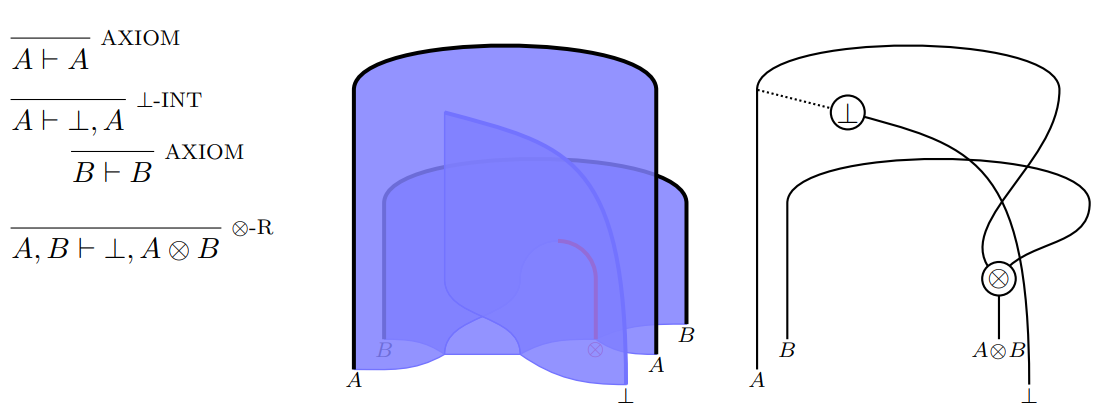
\includegraphics[width=130mm]{pictures/proof_net.png}
%\caption{3D representation of proof nets \cite[Fig. 1]{dunn} }
%\end{figure}
%
%The thinning links (drawn as dotted lines on the right hand side of this figure) can be seen to arise as a way to recover the connectivity information of the units which is lost as degeneracies in the projection from 3 to 2-dimensions.
%
%
%This is an essential difference for proof nets for monoidal categories and proof nets for linearly distributive categories. In particular, monoidal categories can be regarded as special cases of linearly distributive categories where both monoidal structures coincide and the linear distributors are the associators.  In this case, the distributor is redundant, and the 3rd dimension adds no new information. Therefore,  the calculus of thinning links which keeps track of the connectivity information of the units is not needed.  Thus, in the monoidal setting one recovers proof nets we reviewed in the previous subsection.
%
%
%
%On a separate note, linearly distributive categories have also been used to explore quantum causality \cite{sander} as well as to give toy models for infinite dimensional quantum processes  \cite{muc}.  Therefore, there is also motivation for understanding proof nets in the non-monoidal setting in the context of exploring quantum mechanics from a categorical perspective, although it is not the focus of this thesis.



